\documentclass[a4paper]{report}

\usepackage[nocompress]{cite}
\usepackage[utf8]{inputenc}
\usepackage{amsmath}
\usepackage{amsfonts}
\usepackage{amssymb}
\usepackage{amsthm}
\usepackage{graphicx}
\usepackage{url}
\usepackage{subfigure}
\usepackage{multirow}

\usepackage{tikz}
\usepackage{color}
\usetikzlibrary{automata,backgrounds,petri}

\usepackage{algorithmic}
\usepackage{algorithm}
\numberwithin{algorithm}{chapter}

\begin{document}

\addtocontents{lof}{\vspace*{-20pt}}
\addtocontents{lot}{\vspace*{-20pt}}
\addtocontents{loa}{\vspace*{-10pt}}

\newtheorem{thm}{Theorem}[chapter]
\newtheorem*{thm*}{Theorem}
\newtheorem{cor}[thm]{Corollary}
\newtheorem{lem}[thm]{Lemma}

\theoremstyle{remark}
\newtheorem{rem}[thm]{Remark}

\theoremstyle{definition}
\newtheorem{define}[thm]{Definition}
\newtheorem{example}[thm]{Example}
\newtheorem{proposition}[thm]{Proposition}

\newcommand{\proglab}{\textsc{ProgLab}}
\newcommand{\scala}{\textsc{Scala}}
\newcommand{\dabs}{\emph{drop}-abstraction}
\newcommand{\iabs}{$\infty$-abstraction}
\newcommand{\pn}{Petri net}
\newcommand{\pns}{Petri nets}

\newcommand{\HRule}{\rule{\linewidth}{0.5mm}}

\newbox\subfigbox             % Create a box to hold the subfigure.
\makeatletter
\newenvironment{subfloat}% % Create the new environment.
{\def\caption##1{\gdef\subcapsave{\relax##1}}%
    \let\subcapsave=\@empty % Save the subcaption text.
        \let\sf@oldlabel=\label
        \def\label##1{\xdef\sublabsave{\noexpand\label{##1}}}%
        \let\sublabsave\relax    % Save the label key.
        \setbox\subfigbox\hbox
        \bgroup}%              % Open the box...
{\egroup                % ... close the box and call \subfigure.
    \let\label=\sf@oldlabel
        \subfigure[\subcapsave]{\box\subfigbox}}%
        \makeatother

\begin{titlepage}
\begin{center}
% Upper part of the page
\includegraphics{EPFL_logo}\\[1cm]
\textsc{\large Models and Theory of Computation (MTC)}\\[1.5cm]
\textsc{\Large Master Thesis}\\[0.5cm]
% Title
\HRule \\[0.4cm]
{ \huge \bfseries Verification of Concurrent Asynchronous Message passing Programs}\\[0.4cm]
\HRule \\[1.5cm]
% Author and supervisor
\begin{minipage}{0.4\textwidth}
\begin{flushleft} \large
\emph{Author:}\\
Damien Zufferey
\end{flushleft}
\end{minipage}
\begin{minipage}{0.4\textwidth}
\begin{flushright} \large
\emph{Supervisors:} \\
Thomas A. Henzinger\\ Thomas Wies
\end{flushright}
\end{minipage}
\vfill
% Bottom of the page
{\large \today}
\end{center}
\end{titlepage}

\begin{abstract}
Writing concurrent programs is a very delicate task.
%In this context, bugs are hardly reproducible.
The nondeterminism introduced by the scheduler makes bugs in concurrent programs hardly reproducible.
Formal verification can help the programmer to find such bugs.
%We focus on the special case of \scala{} programs that use actors.
In this thesis we focus on actor programs.
Actors provide a model for concurrent programs based on asynchronous message passing.
The contribution of this report is twofold.
First we detail our investigation of \emph{static} systems of actors, i.e. actors programs where the number of created actors is finite and known at compile time.
%More precisely we focus on proving deadlock freedom.
We develop a technique for proving deadlock freedom of such systems.
We achieve a good level of scalability through a heuristic that detects potential deadlocks.
Finally we explore the possibility of extending the static model with dynamic actor creation.
Due to the undecidability of all verification related problems for the general class of system with actor creation, we restrict ourself to certain systems which we call star topologies.
In star topologies, only a finite set of actors can create other actors and the topology is restricted to a star shape, where dynamically created actors cannot communicate with each other.
%The resulting model supports actor creation but with the restriction of having a star topology.
In practice, programs following a client-sever kind of communication fall into this category of star topologies.
%TODO mention scala for examples
\end{abstract}

\tableofcontents
\begingroup
\let\clearpage\relax
  \listoffigures
  \listofalgorithms
  \listoftables
\endgroup

\chapter{Introduction}

%\section{Background}
%Why
The wide availability of multi-core processors makes the need for concurrent programming paradigms more urgent than ever.
A few years ago, buying a new processor was sufficient to ensure that programs execute faster.
Now buying a new processor means that you can execute more applications at the same time, but not necessarily that they will execute faster.
The problem is that most applications are not capable of using the multiple cores available.

\paragraph{}
%What: verification of scala actor
To use these additional processors, programs must be able to execute some of their computations concurrently.
However, writing such programs is a very delicate task.
The result of an execution depends not only on the input, but also on external factors like the scheduler.
In this context, bugs are hardly reproducible.
Formal verification can help the programmer to find such bugs.

\paragraph{Overview of Concurrent Systems.}
There are mainly two paradigms to engineer concurrent programs:

\begin{description}

\item[Shared memory] is a setting where the processes communicate through a single memory that everybody can access.
The synchronisation is done through locks, semaphores, rendezvous, etc.
The more recent development of shared memory are concentrating on software transactional memory.

\item[Message passing] is a setting where the processes communicate only through messages.
The processes do not have any common memory.
The different flavors go from simple unbuffered message exchange between two processes up to group communication primitives (broadcast) in dynamically changing groups.
\end{description}

For multi-core CPU, a program using messages is typically slower than a program using shared memory, because the messages introduce overhead.
On the other hand a program using messages scales to clusters and grid computing.
A shared memory quickly becomes the bottleneck when the number of processors is large.

\paragraph{}
There exist multiple models for message passing concurrency such as
    CCS \cite{DBLP:books/sp/Milner80},
    CSP \cite{DBLP:journals/cacm/Hoare78},
    and Actors \cite{DBLP:conf/ijcai/HewittBS73}.
Some of these models are studied in the context of hardware, where communication is generally synchronized through a bus.
Other models are studied in the context of distributed system, where message passing systems are usually considered to use asynchronous FIFO channels.
In the rest of this work we will consider the Actor model.
This model is a fully asynchronous model with unordered channels.
See Section~\ref{actorModel} for more details.
The actor model is interesting due to its wide-spread use in modern programming languages such as \textsc{Erlang}\cite{DBLP:conf/hopl/Armstrong07} and \scala{}\cite{DBLP:conf/aplas/Odersky04}.

\begin{example}[Actor system]

Figures \ref{ping} and \ref{pong} show a system were two actors play ping-pong together.
The left-hand sides show \scala{} implementations of the involved actors.
The right-hand sides show message-passing automata that we use to graphically represent actors.
%TODO briefly explain the FSM
The notation ``a ? b'' stands for receiving a message b from a, and ``a ! b'' means sending b to a.

The system consists of two actors Ping and Pong that exchange messages.
The Pong actor plays with anybody that sends him a `ball' in the form of a \texttt{Ping} message until he is told to stop.
The Ping actor knows his opponent $pong$.
His behaviour is to send a \texttt{Ping} at the beginning, or when he receives a \texttt{Pong} message.
Ping may also take the decision to end the match and tell $pong$ so by sending a \texttt{Stop} message.

\begin{figure}[ht]
  \centering
\begin{subfloat}
\begin{minipage}[b]{6cm}
{\scriptsize
\begin{verbatim}
class Ping(count: Int, pong: Actor)
    extends Actor {
  def act() {
    var pingsLeft = count - 1
    pong ! Ping
    loop {
      react {
        case Pong =>
          if (pingsLeft % 1000 == 0)
            println("Ping: pong")
          if (pingsLeft > 0) {
            pong ! Ping
            pingsLeft -= 1
          } else {
            println("Ping: stop")
            pong ! Stop
            exit()
          }
      }
    }
  }
}
\end{verbatim}
}
\end{minipage}
\end{subfloat}
\subfigure{
  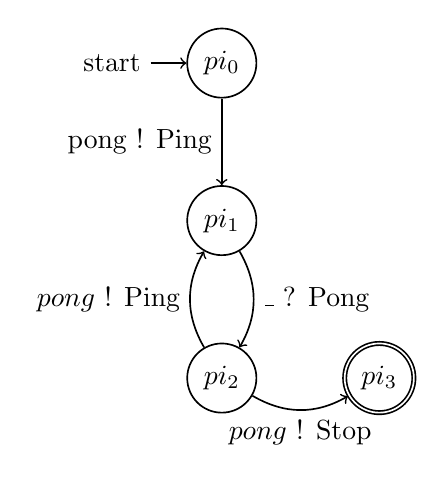
\begin{tikzpicture}[->,auto, node distance=2cm, semithick]
      \node [state,initial] (pi0) {$pi_0$};
      \node [state] (pi1) [below of=pi0] {$pi_1$};
      \node [state] (pi2) [below of=pi1] {$pi_2$};
      \node [state,accepting] (pi3) [right of=pi2] {$pi_3$};
      \path
      (pi0) edge node[left] { pong ! Ping } (pi1)
      (pi1) edge [bend left] node[right] { \_ ? Pong } (pi2)
      (pi2) edge [bend left] node[left] { $pong$ ! Ping } (pi1)
      (pi2) edge [bend right] node[below] { $pong$ ! Stop } (pi3)
      ;
  \end{tikzpicture}
}
  \caption{Ping($pong$)}
  \label{ping}
\end{figure}


\begin{figure}[ht]
  \centering
\begin{subfloat}
\begin{minipage}[b]{6cm}
{\scriptsize
\begin{verbatim}
class Pong extends Actor {
  def act() {
    var pongCount = 0
    loop {
      react {
        case Ping =>
          if (pongCount % 1000 == 0)
            println("Pong: ping "+pongCount)
          sender ! Pong
          pongCount += 1
        case Stop =>
          println("Pong: stop")
          exit()
      }
    }
  }
}
\end{verbatim}
}
\end{minipage}
\end{subfloat}
\subfigure{
  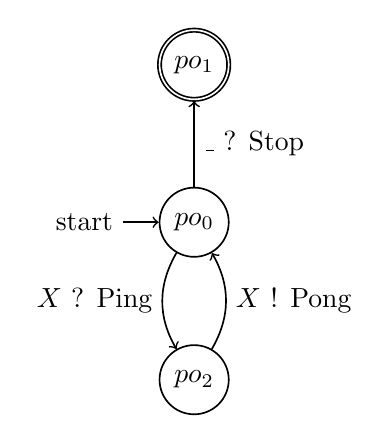
\begin{tikzpicture}[->,auto, node distance=2cm, semithick]
  \node [state,initial] (po0) {$po_0$};
  \node [state,accepting] (po1) [above of=po0] {$po_1$};
  \node [state] (po2) [below of=po0] {$po_2$};
  \path
  (po0) edge node[right] { \_ ? Stop } (po1)
  (po0) edge [bend right] node[left] { $X$ ? Ping } (po2)
  (po2) edge [bend right] node[right] { $X$ ! Pong} (po0)
  ;
  \end{tikzpicture}
}
  \caption{Pong}
  \label{pong}
\end{figure}

\end{example}

\paragraph{Properties of Concurrent Systems.}
Concurrent programming brings the synchronisation issues on top of the problems of single-threaded programs.
In order to avoid such bugs, programs have to satisfy certain properties.
Here are examples of such properties:

\begin{itemize}
\item Safety properties like deadlock freedom, invariants.
Safety properties are violated on \emph{finite} executions.
This kind of properties assert that some bad state is not reachable.

\item Liveness properties like termination, livelock freedom.
Liveness properties are violated on \emph{infinite} executions.
These properties assert that something good eventually happens.
\end{itemize}

%For the moment, we focus on safety properties because they are simpler to check.
%Liveness properties may be later added as an extension of the work on safety.
In this work we focus on the verification of safety properties for actor programs.
Safety properties are in general easier to check than liveness properties and the verification of safety properties is often a preliminary task in the verification of liveness properties.

Message passing systems have specific properties like invariants of the communication topology
(for instance, absence of isolated process in dynamically changing topologies).
These properties can be inferred using appropriate techniques, but this is beyond the scope of this work.

\paragraph{Contributions.}
First we present a possible formalisation of actors in the asynchronous $\pi$-calculus.
It is different from other calculi \cite{DBLP:conf/birthday/AghaT04} in the sense that we focus on the decidability of verification related problems.

Then we identify a \emph{static} subset without creation of actors that reduces to \pns{}.
We present an approximation algorithm for checking deadlock freedom specifically designed for the resulting \pns{}.
We draw inspiration from results about structural analysis of \pns{}, flexible manufacturing systems, and lazy SMT solvers.

Finally, we introduce a new model, which we call star topologies.
Star topologies supports some limited form of actor creation.
In a star topology system, only a finite set of actors can create other actors and the topology is restricted to a star shape, i.e. dynamically created actors cannot communicate with each other.
In practice, programs following a client-sever kind of communication fall into this category.
We give a semi-algorithm to analyse the systems expressed in this new model.
The soundness of the semi-algorithm is proved.
The semi-algorithm uses techniques such as counter abstraction and results about well structured transition systems.

\paragraph{Proof of Concept.}
We implemented some of the analyses presented in this thesis as plug-ins to the \scala{} compiler.
We target programs that use \scala{}'s Actor library \cite{DBLP:conf/jmlc/HallerO06,DBLP:conf/coordination/HallerO07}, which is developed by Pilipp Haller and Martin Odersky.
The actor library has more features than we can currently handle in our model.
%in the scope of this thesis, we restrict ourself to a subset of the library.
However, we support the most commonly used subset of the library: \texttt{!} (send), \texttt{receive/react}, which are both asynchronous, and \texttt{!?}, \texttt{reply}, which can emulate synchronous behaviour.
Methods that have a time constraint or that permit direct interaction with the \texttt{Actor}'s mailbox interfere with the decidability of the models that we use.
Therefore such methods are not allowed.
%The \scala{} compiler has a plug-in system.
%We use it to delegate the job of parsing and typing to the compiler, since we work directly on the abstract syntax tree.
%Moreover, with the Actor library come examples and existing code that we use as benchmarks for our analysis.

\paragraph{Structure of the thesis.}
After introducing some formalism in Chapter \ref{chapPrem}, we recall some of our previous work about modelling actor systems in Chapter \ref{chapModel}.
In Chapter \ref{chapStatic}, we pay attention to a particular subset called static systems.
We use known results from the $A\pi$-calculus and \pns{} to analysis this subset.
Finally, Chapter \ref{chapDynamic} is dedicated to the extended model of star topologies.


\chapter{Preliminaries}
\label{chapPrem}
We now introduce some of the formalism that is used in the later sections of this report.
We also refer to some standard notions such as linear programming (LP), integer linear programming (ILP), and boolean satisfiability (SAT).
We assume that the reader knows the concepts and algorithms related to these problems \cite{decision_procedure}.


\section{$\pi$-calculus}
Informally, the $\pi$-calculus\cite{DBLP:journals/iandc/MilnerPW92a,DBLP:journals/iandc/MilnerPW92b} is considered to be the $\lambda$-calculus of message passing concurrency.
It tries to be minimal, but keeps a great modeling power.
It can model synchronous and asynchronous communication, changing network topologies, dynamic creation of processes, etc.

\paragraph{}
A fundamental concept of the $\pi$-calculus is the notion of names.
Names are very similar to channels, as processes can send and receive messages through them.
Furthermore, names are also first-class values that can be sent and created.

\subsection{Syntax}

In the $\pi$-calculus, a process (formula) $P$ is defined by the following grammar:

\begin{tabular}{lclr}
$P$ & ::= & $x(y).P $                           & (input prefix)\\
    & $|$ & $\overline{x} \langle y \rangle.P $ & (output prefix)\\
    & $|$ & $ \sum_i a_i(b_i).P_i $             & (external choice) \\
    & $|$ & $P\;|\;P $                          & (parallel composition)\\
    & $|$ & $!P $                               & (replication) \\
    & $|$ & $(\nu x)P $                         & (name creation)\\
    & $|$ & $0 $                                & (unit process)
\end{tabular}

\begin{rem}
The \emph{internal choice} a construct which is generally used to encode nondeterministic branching is omitted in the above definition.
However, it can be emulated using the following construct:
\begin{equation*}
A \oplus B \Leftrightarrow (\nu a)(\nu b)(\overline{a} \;|\; \overline{b} \;|\; a().A + b().B )
\end{equation*}
Or by a construct without channel creation:
\begin{equation*}
A \oplus B \Leftrightarrow (\overline{a} \;|\; \overline{b} \;|\; a().b().A + b().a().B )
\end{equation*}
if $a$ and $b$ are not used anywhere else.
\end{rem}

\subsection{Operational semantics}

We call \emph{threads} the subformula separated by `$|$'.
Informally threads are doing the computations in a $\pi$-calculus process.%, they define the system's behaviour.
On the other hand, the \emph{names} give the topology of the `network' of threads.
They do not perform computations, but are the support for the messages.

\noindent
Here is an informal description of the types of formula in the grammar:\\
{\centering
\begin{tabular}{lp{9cm}}
\hline
\hline
$x(y).P$ & means that a name is received from $x$, bound to $y$, and the process continues as $P$. \\
\hline
$\overline{x} \langle y \rangle.P$ & means that the name $y$ is send on $x$ and the process continues as $P$. \\
\hline
$\sum_i a_i(b_i).P_i $ & receive one of the available messages or blocks when there is no message at all.\\
\hline
$P_1\;|\;P_2$ & denotes the concurrent execution of $P_1$ and $P_2$. \\
\hline
$!P$ & means that $P$ can be replicated as many time as needed.\\
\hline
$(\nu x)P$ & creates a new fresh name $x$ in the scope of $P$.\\% $x$ is a normal channel and can be used as such. \\
\hline
$0$ & is a process whose execution is finished.\\
\hline
\hline
\end{tabular}
}

\paragraph{}
Here is a \emph{partial} overview of the evaluation of a $\pi$-calculus process.
The evaluation mixes the application of reduction rules and congruence rules.
The reduction rules are detailed in Table \ref{tblPiRed} and the congruence rules in Table \ref{tblPiCong}.
The first two reduction rules are the most important as they corresponds to the reception of a message.
For more details, refer to \cite{DBLP:books/sp/Milner80,DBLP:journals/iandc/MilnerPW92a,DBLP:journals/iandc/MilnerPW92b}

\begin{table}
\caption{Reduction rules for $\pi$-calculus}
\label{tblPiRed}
\centering
\begin{eqnarray*}
& \overline{x}\langle z \rangle.P \;|\; x(y).Q \rightarrow P \;|\; Q[z/y] \\
&\overline{a}\langle b \rangle.P \;|\; \sum_{i \in I} a_i(b_i).Q_i ~~ \rightarrow ~~ P \;|\; Q_x[b/b_x] ~~~~ \text{where $a_x = a$}\\
&P \rightarrow Q \Rightarrow P\;|\;R \rightarrow Q\;|\;R \\
&P \rightarrow Q \Rightarrow (\nu x)P \rightarrow (\nu x)Q \\
&P \equiv P^\prime \land Q \equiv Q^\prime \land \rightarrow Q \Rightarrow P^\prime \rightarrow Q^\prime
\end{eqnarray*}
\end{table}

\begin{table}
\caption{Congruence rules for $\pi$-calculus}
\label{tblPiCong}
\centering
\begin{tabular}{c c}
 & \\
$P\;|\;Q \equiv Q\;|\;P$ & $P\;|\;0 \equiv P$ \\
$(P\;|\;Q)\;|\;R \equiv P\;|\;(Q\;|\;R) $ & $(\nu x)(\nu y)P \equiv (\nu y)(\nu x)P$ \\
$(\nu x)0 \equiv 0 $ & $\sum_{i \in \emptyset} a_i(b_i).Q_i \equiv 0$ \\
$\sum_{i \in \{x\}} a_i(b_i).Q_i \equiv a_x(b_x).Q_x$ & $!P \equiv \; !P\;|\;P$ \\
\multicolumn{2}{c}{$P \equiv Q$ if $Q$ can be obtained from $P$ by renaming bound names in $P$.}\\
\multicolumn{2}{c}{$(\nu x)(P | Q) \equiv (\nu x)P | Q$ if $x$ is not a free name of $Q$.}
\end{tabular}
\end{table}


\section{Petri Nets}
\pns{} are a modeling language for discrete distributed systems.
They were invented by Carl Adam Petri when he was only 13 years old \cite{pn}.
A \pn{} is a directed bipartite graph where the nodes are divided in \emph{places} and \emph{transitions}.
Places may contains some tokens, that are consumed and created by transitions.
We give a brief introduction into \pns{}.
For a detailed introduction see, e.g., \cite{fcbook,DBLP:journals/eik/EsparzaN94,DBLP:conf/ac/Esparza96}.

\paragraph{Notations.}
A \pn{} is a 4-tuple $(S,T,F,M)$, where $S$ and $T$ are finite sets of places and transitions.
$F \; \subseteq \; (S \times T) \bigcup (T \times S) \rightarrow \{0,1\}$ is the flow relation.
$M: S \rightarrow \mathbb{N}$ is the current marking.
The \emph{preset} $\bullet x$ and \emph{postset} $x \bullet$ of a place or transition $x$ are defined as
$ \bullet x = \{ y | (y,x) \in F\}$ and
$ x \bullet = \{ y | (x,y) \in F\}$.

A transition $t$ is enabled at $M$ if $M(s) > 0$ for all $s \in \bullet t$.
When a transition is enabled it can fire (sometimes we also say it occurs).
The firing of $t$ leads to marking $M^\prime$, where $M^\prime(s) = M(s) + F(t,s) - F(s,t)$.
We denote by $M \buildrel t \over \longrightarrow  M^\prime $ the firing of $t$ in $M$.

\paragraph{}
A survey for \pns{} decidability and complexity for different problem can be found in \cite{DBLP:journals/eik/EsparzaN94}.
Problems like covering, liveness of transitions, reachability for \pns{} are decidable, but very expensive (EXPSPACE-hard \cite{DBLP:conf/stoc/CardozaLM76}).


\chapter{Modeling Actor Systems}
\label{chapModel}
This chapter introduces the Actor model.
We explain how to formalise it in the asynchronous $\pi$-calculus.

\section{The Actor Model}
\label{actorModel}
This part is a brief introduction to the Actor model
\footnote{This part is inspired by \url{http://en.wikipedia.org/wiki/Actor_model}, a very complete article.}.

\paragraph{}
The Actor model serves as a theoretical model for message passing concurrency.
It was originally proposed by Hewitt, Bishop, and Steiger \cite{DBLP:conf/ijcai/HewittBS73}.
Later work includes \cite{WilliamClinger81,GulAgha86}.

An actor is a `process' that can in each transition:
\begin{itemize}
\item send finitely many messages to other actors.
\item create a finite number of new actors.
\item receive a message from its mailbox and continue with a specified behaviour.
\end{itemize}

Sending a message is an asynchronous action.
The actor does not wait for someone to receive it.
When multiple messages are waiting in the mailbox, the delivery order is not specified.
In practice, most implementations based on the Actor model use many-to-one queues as the underlying data structure for mailboxes.

\section{Choosing the Right Formalism}
One critical step in program analysis is finding a model that is suitable for the verification task at hand.
Using the right mathematical formalism helps identifying and solving the problems that will eventually arise.

The Actor model \cite{DBLP:conf/ijcai/HewittBS73,WilliamClinger81,GulAgha86} provides a clear semantics for message passing concurrency, but it is not a process calculus.
%TODO it is easier to work with a process calculus 
A general implementation of the capabilities of the model is Turing complete.
Since we want to have algorithms to solve safety problems related to actors, we are interested in identifying subsets where the reachability problem is decidable.

If we consider only synchronous message passing then, without actor creation, the reachability problem is clearly decidable because nothing is unbounded.
However, it is not well suited to model actors: asynchronous message passing is an essential feature of actors.
It is possible to insert a buffer process to simulate a mailbox, but then we have to consider actors with infinite state-space.
This addition brings more problems than it solves.

The \scala{} actors' library implements mailboxes with queues.
A queue is an unbounded linear memory.
Therefore, as soon as there is more than one actor, it is possible to encode a Turing machine \cite{DBLP:journals/jacm/BrandZ83}.

By relaxing the ordering on the messages in the mailbox, it is possible to be decidable again.
This follows from results about the $A\pi$-calculus \cite{DBLP:journals/njc/AmadioM02}.
Therefore, we consider the following model for our actor systems: \emph{Asynchronous message-passing model with multisets as mailbox}.
%Implementing mailboxes with queues is the closer to \scala{} implementation, but using multisets is closer to the original Actor model.
%TODO ...
The behaviour of one actor is expressed as a finite state machine where the edges are annotated with operations, as seen in Figures \ref{ping} and \ref{pong}. 
We now give a formal definition of actor programs in terms of the $\pi$-calculus.

\begin{rem}
Simple finite state machines are used to model the control flow because adding recursion to the model makes it undecidable\cite{DBLP:journals/toplas/Ramalingam00}.
\end{rem}

\section{Actors in the $A\pi$-calculus}

The features of the actor model are easily expressible in the $\pi$-calculus.
\begin{itemize}
\item The mailboxes correspond to names.
\item The actors correspond to threads.
\item Sending a message corresponds to an output prefix.
\item Receiving a message corresponds to an input prefix.
\item Parallel composition models the simultaneous execution of multiple actors.
\end{itemize}

\begin{example}
Two actors playing ping-pong expressed as one $\pi$-calculus process:
\begin{equation*}
(\nu p_{ing})(\nu p_{ong}) !( \overline{p_{ong}}\langle p_{ing} \rangle. p_{ing}(p_{ong}). 0 )
                     \;|\; !( p_{ong}(p_{ing}). \overline{p_{ing}}\langle p_{ong} \rangle. 0 )
\end{equation*}
\end{example}


The $\pi$-calculus has even ``too much'' features for our need.
For instance, we do not use synchronous message exchanges.
Using a version of the calculus where some of the unneeded features are not present keeps the formalism simpler.

\paragraph{$A\pi$-calculus.}
In order to model actors, we use a restricted version of the $\pi$-calculus known as the \textit{asynchronous} $\pi$-calculus \cite{DBLP:conf/ecoop/HondaT91,Boudol92asynchronyand}, or $A\pi$-calculus.
In the $A\pi$-calculus, the output \emph{prefix} does not exist.
This means that after sending a message, the sending thread always continues as the unit process.
In other words, there is no way to know when a message is delivered.
Therefore no synchronous communication is possible.

\paragraph{}
To translate the example from previous section to the $A\pi$-calculus fragment:\\
$( \overline{p_{ong}}\langle p_{ing} \rangle. p_{ing}(p_{ong}). 0 )$
has to be replaced by
$( \overline{p_{ong}}\langle p_{ing} \rangle. 0 \;|\; p_{ing}(p_{ong}). 0 )$

\paragraph{General system of actors.}

There are five different operations that an actor can perform:
\begin{itemize}
\item Receiving a message;
\item Sending a message;
\item Branching;
\item Creating a new channel;
\item Creating a new actor.
\end{itemize}

%TODO transition
In the $A\pi$-calculus, the notion of threads and channels are completely separated.
In the actor model, a channel is attached to a specific actor.
Channels are many-to-one only.
A syntactic restriction, the unique receiver condition \cite{DBLP:journals/tcs/Amadio00,DBLP:journals/njc/AmadioM02}, guarantees that channels are not shared.
In order to enforce this property, names are separated into two groups.
One group $\vec a_I$ represents the names owned by one actor.
It is possible to receive only from an owned name.

For each operation we give a formula with the appropriate semantic.
\begin{eqnarray}
\label{receive}     P(\vec a_I; \vec a_O) & = & \sum_{i \in I} a_i (\vec{b_i}).P_i(\vec a_I ;\vec a_O, \vec b_i) \hspace{7mm} \forall i \in I, a_i \in a_I \\
\label{send}        P(\vec a_I; \vec a_O) & = & \overline{a}\langle \vec{b} \rangle | P^\prime(\vec a_I ;\vec a_O) \\
\label{choice}      P(\vec a_I; \vec a_O) & = & A(\vec a_I; \vec a_O) \oplus B(\vec a_I; \vec a_O) \\
\label{channel}     P(\vec a_I; \vec a_O) & = & (\nu \vec a).P^\prime(\vec a_I, \vec a; \vec a_O) \\
\label{creation}    P(\vec a_I; \vec a_O) & = & (\nu \vec n)(Q(\vec n;\emptyset) | P^\prime(\vec a_I ; \vec a_O , \vec n)) 
\end{eqnarray}
In all of the equations (\ref{receive})-(\ref{creation}), we assume that all the input parameters $\vec a_I$ are distinct.
The continuations in the equations above are the \emph{maximal} set of possible parameters.
In practice, the parameters of the continuations are often only a subset of what is allowed.

\begin{define}[Actor]
\label{defActor}
An \emph{actor} $A = (\mathit{def},\mathit{state})$ is a pair of :
\begin{itemize}
\item $\mathit{def}$ is a finite set of mutually recursive equations of the form (\ref{receive}), (\ref{send}), (\ref{choice}), (\ref{channel}), and (\ref{creation}).
These formulas define the behaviour of $A$.
\item $\mathit{state}$ is an equation in $\mathit{def}$ where some parameters might be instantiated.
\end{itemize}
\end{define}

\begin{define}[Free Parameter]
\label{defFreeParam}
The \emph{free parameters} of an actor are the free parameters of the equations that compose this actor.
\end{define}

\begin{define}[System]
\label{defSys}
An actor \emph{system} is a finite set $S$ of actors (Definition \ref{defActor}).
The system behaves as the $A\pi$-calculus equation:
\begin{equation*}
\prod_{(\mathit{def},\mathit{state}) \in S} \mathit{state}
\end{equation*}
\end{define}

\begin{rem}
$\prod$ is a shorthand for $|$ likewise $\sum$ is a shorthand for +.
\end{rem}

\subparagraph{Equations as control flow locations.}
It is possible to interpret the system of mutually recursive equations as a edge-labeled finite state machine \emph{CFA}.
Notice that every equation has only one continuation (except for messages).
Let each equation $e$ corresponds to a location $l$ of \emph{CFA}.
For each continuation $c$ in the equation $e$, create an edge from $l$ to $c$ with the appropriate label (send,receive,$\epsilon$).
Figures \ref{piPing}, \ref{piPong} give examples of actors with their automata form.


\begin{figure}[ht]
  \centering
\subfigure{
\begin{minipage}[b]{6cm}
\begin{eqnarray*}
pi_0    & = & \overline{\text{pong}_{Ping}}\langle \text{ping}_{Pong} \rangle | pi_1\\
pi_1    & = & \text{ping}_{Pong}().pi_2 \\
pi_2    & = & pi_{2a} \oplus pi_{2b} \\
pi_{2a} & = & \overline{\text{pong}_{Ping}}\langle \text{ping}_{Pong} \rangle | pi_1\\
pi_{2b} & = & \overline{\text{pong}_{Stop}}\langle \rangle | pi_3 \\
pi_3    & = & 0
\end{eqnarray*}
\mbox{}\\
\mbox{}\\
\end{minipage}
}
\subfigure{
  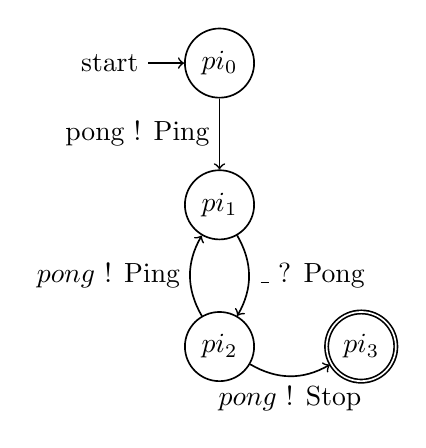
\begin{tikzpicture}[->,auto, node distance=18mm, semithick]
      \node [state,initial] (pi0) {$pi_0$};
      \node [state] (pi1) [below of=pi0] {$pi_1$};
      \node [state] (pi2) [below of=pi1] {$pi_2$};
      \node [state,accepting] (pi3) [right of=pi2] {$pi_3$};
      \path
      (pi0) edge node[left] { pong ! Ping } (pi1)
      (pi1) edge [bend left] node[right] { \_ ? Pong } (pi2)
      (pi2) edge [bend left] node[left] { $pong$ ! Ping } (pi1)
      (pi2) edge [bend right] node[below] { $pong$ ! Stop } (pi3)
      ;
  \end{tikzpicture}
}
  \caption{Ping in $A\pi$-calculus}
  \label{piPing}
\end{figure}


\begin{figure}[ht]
  \centering
\subfigure{
\begin{minipage}[b]{6cm}
\begin{eqnarray*}
po_0    & = & \text{pong}_{Stop}().po_1 \\
        & + & \text{pong}_{Ping}(X).po_2\\
po_1    & = & 0 \\
po_2    & = & \overline{X}\langle \rangle | po_0
\end{eqnarray*}
\mbox{}\\
\mbox{}\\
\end{minipage}
}
\subfigure{
  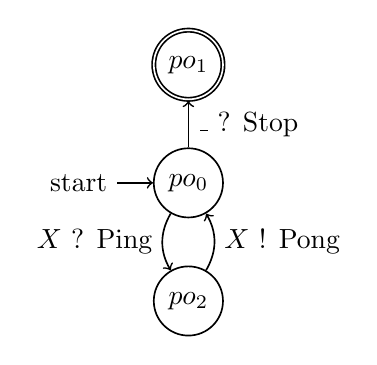
\begin{tikzpicture}[->,auto, node distance=15mm, semithick]
  \node [state,initial] (po0) {$po_0$};
  \node [state,accepting] (po1) [above of=po0] {$po_1$};
  \node [state] (po2) [below of=po0] {$po_2$};
  \path
  (po0) edge node[right] { \_ ? Stop } (po1)
  (po0) edge [bend right] node[left] { $X$ ? Ping } (po2)
  (po2) edge [bend right] node[right] { $X$ ! Pong} (po0)
  ;
  \end{tikzpicture}
}
  \caption{Pong in $A\pi$-calculus}
  \label{piPong}
\end{figure}

\chapter{Deadlock Freedom of Static Actor Systems}
\label{chapStatic}
In this chapter, we define a subset of the actor model that corresponds to a decidable fragment of the $A\pi$-calculus.
This fragment reduces to \pns{}.
Unfortunately, most problems for \pns{},including the reachability problem, are EXPSPACE-hard.
For this reason we concentrate on a more specific problem, namely deadlock-freedom, and develop a sound but approximative solution.
This approximative solution is based on a well-known necessary condition for deadlock and works by examining the structure of the net.

In the following, we first define static actor systems.
Then we explain how to adapt the proof of EXPSPACE-hardness of the reachability problem for \pns{} to prove the EXPSPACE-hardness of the reachability problem for static actor systems.
After that we recall useful structural properties of \pns{}.
With the help of these properties, a sufficient condition for deadlock freedom, and drawing inspiration from lazy SMT solvers\cite{Moura02lemmason}, we develop our approximative solution.

\section{Static Actor Systems}

\paragraph{Decidability of the $A\pi$-calculus.}
The reachability problem is not decidable in the full $A\pi$-calculus.
But with some restrictions it is possible to be decidable again \cite{DBLP:journals/njc/AmadioM02}.
In our case, we choose not to allow name creation.
In terms of actors, this means that dynamic creation of actors and channels is not allowed.

This fragment without name creation reduces to \pns{} and its analysis uses existing algorithms.
Later we will introduce other fragments that contains more operations.

\subparagraph{}
We use equations with a sightly different shape compared to \cite{DBLP:journals/njc/AmadioM02}.
But both forms are equivalents.
In this fragment, we allow equation of the following kind:
\begin{eqnarray}
\label{static_receive}  \text{receiving} & : & \sum_{i \in I} a_i (\vec{b_i}).P_i \\
\label{static_send}     \text{sending} & : &    \overline{a}\langle \vec{b} \rangle | P \\
\label{static_choice}   \text{branching} & : &    A \oplus B
\end{eqnarray}

\begin{define}[Static Actor]
\label{defStaticActor}
An \emph{static actor} $A = (\mathit{def},\mathit{state})$ is a pair of :
\begin{itemize}
\item $\mathit{def}$ is a finite set of mutually recursive equations of the form (\ref{static_receive}), (\ref{static_send}), and (\ref{static_choice}).
These formulas define the behaviour of $A$.
\item $\mathit{state}$ is an equation in $\mathit{def}$ where some parameters might be instantiated.
\end{itemize}
\end{define}

\begin{define}[Static system]
\label{defStaticSys}
A \emph{static system} is a finite set $S$ of static actors (Definition \ref{defStaticActor}).
The system is static because the actors are not able to create new actors.
It behaves as the $A\pi$-calculus equation:
\begin{equation*}
\prod_{(\mathit{def},\mathit{state}) \in S} \mathit{state}
\end{equation*}
\end{define}


\subsection{Translating static systems to \pns{}}

As stated before, it is possible to use algorithms for the analysis of \pns{} as back-end for the analysis of actors systems.
The details of the translation from $A\pi$-calculus to \pns{} can be found in \cite{DBLP:journals/njc/AmadioM02}.
Here, we just present the idea with one example.

Consider the ping-pong example given in Figure~\ref{simplePP}.
In it as simplified version of Figures \ref{ping}, \ref{pong}.
The removed parts are greyed.
One possible translation of this static system into a \pn{} is given in Figure~\ref{petri}.
The net can roughly be divided into three parts: the control location of the ping actor, mailboxes, the control location of the pong actor.

\begin{figure}[ht]
  \centering
  \subfigure{
  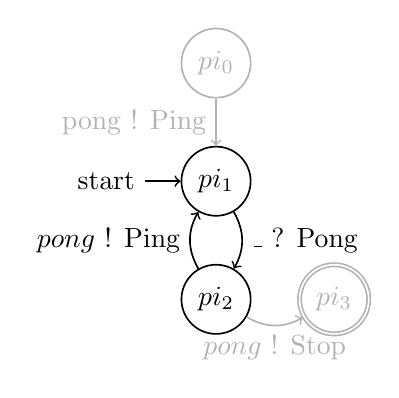
\begin{tikzpicture}[->,auto, node distance=15mm, semithick]
    \node [state,color=black!30] (pi0) {$pi_0$};
    \node [state,initial] (pi1) [below of=pi0] {$pi_1$};
    \node [state] (pi2) [below of=pi1] {$pi_2$};
    \node [state,accepting,color=black!30] (pi3) [right of=pi2] {$pi_3$};
    \path
    (pi0) edge [color=black!30] node[left] { pong ! Ping } (pi1)
    (pi1) edge [bend left] node[right] { \_ ? Pong } (pi2)
    (pi2) edge [bend left] node[left] { $pong$ ! Ping } (pi1)
    (pi2) edge [bend right,color=black!30] node[below] { $pong$ ! Stop } (pi3)
    ;
  \end{tikzpicture}
  }

  \subfigure{
  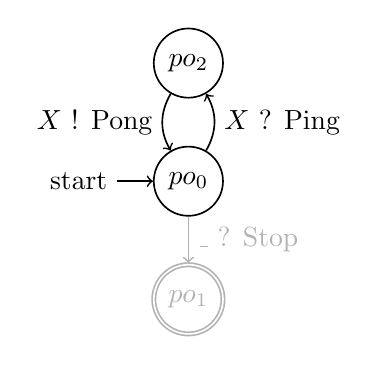
\begin{tikzpicture}[->,auto, node distance=15mm, semithick]
    \node [state,initial] (po0) {$po_0$};
    \node [state,accepting,color=black!30] (po1) [below of=po0] {$po_1$};
    \node [state] (po2) [above of=po0] {$po_2$};
    \path
    (po0) edge [color=black!30] node[right] { \_ ? Stop } (po1)
    (po0) edge [bend right] node[right] { $X$ ? Ping } (po2)
    (po2) edge [bend right] node[left] { $X$ ! Pong} (po0)
    ;
  \end{tikzpicture}
  }
  \caption{Simplified ping-pong}
  \label{simplePP}
\end{figure}

\paragraph{Program state.}
For each location in the control flow graph of an actor there is a corresponding place in the net.
In our setting no actor creation is done, therefore there are nice place invariants\footnote{Place invariants are defined later in Section \ref{defPI}.}
which express that an actor is only at one position in its control flow graph.

\noindent
Let $P = (S,T,F,M)$ be a \pn{} representing a set of actors $S$ then
\begin{equation*}
\sum_{p \in \mathit{def}} M(p) = 1, \forall (\mathit{def}, \mathit{state}) \in S
\end{equation*}
is an invariant of $P$.

\paragraph{Mailboxes.}
There is a ``mailbox place'' per channel and per kind of message that can be sent.
To respect the asynchronous aspect of actors, we model mailboxes explicitly.
Having distinct mailboxes provides a simple way to encode external choice for an actor
\footnote{An external choice is a decision made by something the actor cannot influence. For instance, the messages it receives}.
The number of mailbox places is finite, since there are only finitely many message kinds and actors in a static system.

\paragraph{Free parameters.}
When an equation has free parameters, a case split is done.
A free parameter can take a new value only when a name is received.
At that point, all possible valuations are explored.
This also means that the mailboxes have to be split further because we also need to remember the parameter inside the message (e.g. sender).


\begin{figure}[!ht]
  \centering
  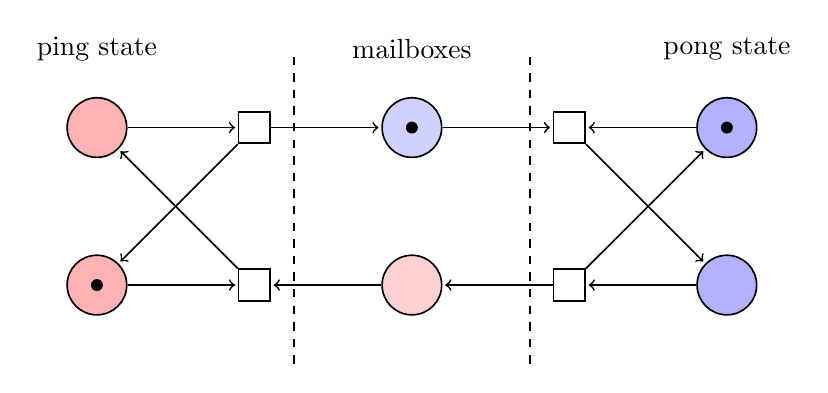
\begin{tikzpicture}[auto, node distance=2cm, semithick]

  \node (label1) at (-4,3) {ping state};
  \node (label2) at ( 0,3) {mailboxes};
  \node (label3) at ( 4,3) {pong state};
  \draw[dashed] (-1.5,-1) -- (-1.5,3);
  \draw[dashed] (1.5,-1) -- (1.5,3);

  
  \node [place,fill=red!18] (ping) at (0,0) {};
  \node [place,tokens=1,fill=blue!18] (pong) [above of= ping] {};

  \node [transition] (pongCatch) [right of= pong] {};
  \node [transition] (pongSend)  [below of= pongCatch] {};
  \node [place,tokens=1,fill=blue!30] (po0) [right of= pongCatch] {};
  \node [place,fill=blue!30] (po1) [below of= po0] {};
  
  \node [transition] (pingCatch) [left of = ping] {};
  \node [transition] (pingSend) [above of= pingCatch] {};
  \node [place,tokens=1,fill=red!30] (pi0) [left of= pingCatch] {};
  \node [place,fill=red!30] (pi1) [above of= pi0] {};
  
  \path
    (pingCatch) edge [pre] (pi0)
                edge [pre] (ping)
                edge [post] (pi1)
    (pingSend)  edge [pre] (pi1)
                edge [post] (pi0)
                edge [post] (pong)
    (pongCatch) edge [pre] (po0)
                edge [pre] (pong)
                edge [post] (po1)
    (pongSend)  edge [pre] (po1)
                edge [post] (po0)
                edge [post] (ping)
  ;

  \end{tikzpicture}
  \caption{\pn{} for simplified ping-pong example}
  \label{petri}
\end{figure}

\section{Lower Bound of Complexity.}

\begin{thm}
Given a static actor system $S$ and a configuration $c$.
The problem of determining whether $c$ is reachable in $S$ is EXPSPACE-hard.
\end{thm}

\begin{proof} (\textit{Sketch})
In \cite{Lipton76,DBLP:conf/ac/Esparza96} a proof for EXPSPACE-hardness of the reachability problem for \pns{} is given by a reduction from bounded counter automaton to \emph{net programs} and then to \pns{}.
We adapt this proof to show that the reachability problem for static actor systems is also EXPSPACE-hard.
We give a polynomial reduction from net programs to static actor systems.

%A net program is like counter automaton, but for the capability to test a counter value.
A net program is a finite set of procedures (one designated as the main procedure where the execution starts).
Each procedure consists of statements that increment or decrement counters and non-recursive calls to other procedures.
Counters cannot be tested for 0.
For a formal definition of net programs see \cite{Lipton76,DBLP:conf/ac/Esparza96}.

When a net program attempts to decrement a counter with value 0, the net program blocks.
%The mailboxes behaves similarly.
Actors behave similarly \emph{w.r.t.} their mailbox than a net program \emph{w.r.t.} counters.
When receiving from an empty mailbox, the actor blocks.
Incrementing a counter in a net program corresponds to sending a message in an actor system.

Net programs have non-recursive procedure calls.
We need to keep them for the complexity analysis.
It is possible to emulate procedure calls, with messages.
a dynamic topology can be used to pass the operands and the return destination of the subroutine calls.
Once the ``call'' was sent, the actor waits for the return message.
Subroutines are actors that wait for a message to start.
When they are finished, they send a return message and return in their starting state.

The \texttt{halt} primitive is replaced by a HALT message sent to a halt actor.
A HALT message is received iff the net program has halted.
Table \ref{tableOp} summarizes the transformation of operations.
\end{proof}

\begin{table}
\caption{Net program operations translated for actor and $A\pi$-calculus}
\label{tableOp}
\centering
\begin{tabular}{|c|c|c|}
\hline
\emph{net program} & Actor & $A\pi$-calculus \\
\hline
\hline
\texttt{x := x + 1}             & self ! X                          & $\overline{\text{self}_X} \langle \rangle$  \\
\texttt{x := x - 1}             & \_ ? X                            & $\text{self}_X () $\\
\texttt{goto $l$}               & $\epsilon$ transition             & $l$ \\
\texttt{goto $l_1$ or $l_2$}    & two transitions from one state    & $l_1 \oplus l_2$ \\
\texttt{gosub $l$}              & $l$ ! (args,return)               & $\overline l \langle \text{args,return} \rangle$ \\
\texttt{return}                 & return ! Done                     & $\overline{\text{return}} \langle \rangle$ \\
\texttt{halt}                   & halt ! HALT                       & $\overline{\text{halt}_{\text{HALT}}} \langle \rangle$\\
\hline
\end{tabular}
\end{table}

\section{Sufficient Condition for Deadlock Freedom}

\paragraph{Focusing on deadlock.}
In order to solve some practical safety problems for static actor systems despite the high complexity of the reachability problem, we focus on a more specific property of concurrent systems: deadlock freedom.
With deadlock in mind, we decide to drop completeness for a faster algorithm.
Obviously, we want to retain soundness, but a complete analysis seems intractable.
We implemented a prototype that translates \scala{} actor programs into \pns{} and uses existing \pn{} algorithms to check deadlock freedom.
In our experiments, we obtained nets that consisted only of a few tenths of states and transitions, yet, their analysis lasted for hours.

%explain in more details the translation + modification of the system to make accepting run infinite
The deadlock property requires a slight modification of the analysed system.
A system in which all actors have successfully finished their computation is in a deadlocked state.
This specific final deadlock is something we wish to eliminate because it corresponds to a normal termination of the program.

\label{placeFinish}
A simple solution to this problem is to add a new designated \emph{finish} place with a loop transition back to itself.
Then for each actor we keep track of which places correspond to an accepting place (i.e. a normal termination).
Without loss of generality it is possible to transform the actor such that it has only one accepting place.
The last step of the transformation is to connect the \emph{finish} place with the rest of the system.
In order to do so, we add a transition that reads from the accepting place of every actor and puts a token in \emph{finish}.

\subsection{Necessary condition for deadlock in \pns{}}
We start from a necessary condition for deadlocks on \pns{} that is defined in terms of structural properties of \pns{}.

\paragraph{Structural properties of \pns{}}
In the study of deadlocks in \pns{}, two structural properties have a prevalent role: \emph{siphons} and \emph{traps}.
Invariants are also useful.

\begin{description}
\item[]A \textbf{Siphon} is a set of places $S$ such that $ \bullet S \subseteq S \bullet $.
A siphon has the property that it cannot receive tokens once it is emptied.
\item[]A \textbf{Trap} is a set of places $T$ such that $ T \bullet \subseteq \bullet T $.
A trap cannot be emptied once it contains tokens.
\item[]A \textbf{Place invariant ($I$,$X$)} is a vector $I$ of integer coefficient such that at least one coefficient is different from 0 and an integer $X$.
For all marking $M$ reachable from $M_0$, the following property holds:
\begin{equation}
\sum_{p \in P} I(p) \cdot M(p) = X
\end{equation}
\label{defPI}
\end{description}

\paragraph{Condition\cite{Commoner72,fcbook}:}
Given a \pn{} $P$ in a deadlocked state (i.e. no transition can fire), there exists an empty siphon covering all the transitions.
As the system is in a deadlock, for each transition there is at least one empty incoming place.
Choosing one of these places for each transition gives a siphon because it covers \emph{all} the transitions of $P$.
Hence the existence of a potentially empty global siphon is a necessary condition for deadlock.
Therefore if no marking with such a siphon is reachable the system is deadlock-free.

\subsection{Checking for emptiness of siphons}
\label{checkSiphon}

In the following we present several sufficient conditions to check that a siphon cannot become empty:
\begin{description}
\item[Initially marked trap.] 
We saw that a trap that is marked can never become empty.
Thus, a siphon containing an initially marked trap will stay marked forever.
Given a set of places there is a polynomial algorithm that returns the maximal trap contained in that set.
Sine traps are closed under union, the maximal trap contains all the traps in the siphon.
Thus it is sufficient to check that the maximal trap is marked \cite{Commoner72,fcbook}.
The algorithm \ref{algMaxTrap} computes in polynomial time the maximal trap included in a siphon.

\begin{algorithm}
\caption{Maximal trap inside a siphon}
\label{algMaxTrap}
\begin{algorithmic}
\REQUIRE $P = (S,T,F,M)$ a petri net, $R \subseteq S$ a set of places %input
\ENSURE returns the maximal trap in $Q \subseteq R$ %output
\STATE $Q \leftarrow R$
\WHILE{$\exists s \in Q, t \in s\bullet $ such that $t \notin \bullet Q $}
\STATE $Q \leftarrow Q \setminus \{s\}$
\ENDWHILE
\RETURN $Q$
\end{algorithmic}
\end{algorithm}

\item[Invariant controlled siphon.]
If a siphon admits an invariant ($I$,$X$) such that $X$ is not 0 then the siphon will never be empty \cite{DBLP:conf/apn/LautenbachR94,DBLP:journals/tsmc/LiZ08}.\\
A siphon $S$ admits an invariant ($I$,$X$) if 
\begin{eqnarray}
&&\text{($I$,$X$) is an invariant of the net;}\\
&&\label{inv_ctrl_siphon} \forall p \in P \land p \notin S, I(p) = 0
\end{eqnarray}
%justify by looking at the form of the system ...
Such a siphon is called an invariant controlled siphon.
They can be found using Algorithm \ref{algInvCtrl}.

\begin{algorithm}
\caption{Invariant controlling a siphon}
\label{algInvCtrl}
\begin{algorithmic}
\REQUIRE $P = (S,T,F,M)$ a petri net, $R \subseteq S$ a siphon %input
\ENSURE returns an invariant controlling $R$ or \texttt{None} %output
\STATE $W \leftarrow $ transition matrix where $w_{s,t} = F(t,s) - F(s,t)$
%\STATE $I$ vector of variables
\STATE problem $\leftarrow \left|
\begin{array}{lrl}
Min ~~ 0 & &\\
\text{subject to:} & I^T \cdot W = 0 & \\
 & I^T \cdot M > 0 & \\
 & I(p) \leq 0 & \forall p \in P \setminus R
\end{array} \right.$
\IF{ LP-solve(problem) }
\RETURN $(I, \sum_{p \in P} I(p) \cdot M(p) )$
\ELSE
\RETURN \texttt{None}
\ENDIF 
\end{algorithmic}
\end{algorithm}

\item[Emptiness as an ILP problem.]
It is possible to encode an over approximation of a \pn{} into an ILP problem.

%general ILP
Given a \pn{} $(S,T,F,M)$, let
\begin{itemize}
\item $\vec p$ be a vector of positive integer variables such that each element of the vector corresponds to the number of tokens in a place of $S$.
$\vec p$ is a vector representation of $M$.
\item $W$ be the ($|S| \times |T|$) transition matrix,\\
where $w_{s,t} = F(t,s) - F(s,t) = [s \in t \bullet] - [s \in \bullet t]$
\item $\vec t$ be a vector of positive integer variable such that each element of the vector corresponds to the number of time a transition is taken.
\end{itemize}
Then define the ILP:

\begin{equation}
\label{ilp_general}
W \vec t = \vec p_{final} - \vec p_{initial}
\end{equation}

The ILP (\ref{ilp_general}) is an approximation of the reachability of configuration $\vec p_{final}$ from $\vec p_{initial}$.
The abstraction made by the ILP problem is that tokens can be consumed before they are produced.
In terms of \pns{}, this approximation lifts the restriction that a place has to contain only a positive number of tokens.

%define the system.
\begin{equation}
\label{ilp_siphon}
\text{Given a \pn{}} \, P ~ \text{and a siphon} \, S: ~~
  W \vec t = \left\{ \begin{array}{ll}
         -p_{initial}(i) & \mbox{if $i \in S$};\\
         free & \mbox{else}.\end{array} \right.
\end{equation}

The ILP (\ref{ilp_siphon}) for an empty siphon is a sightly more relaxed version of the program (\ref{ilp_general}):
If this program does not admit a solution then the siphon $S$ cannot become empty in $P$.
Algorithm \ref{algILPApprox} summarizes this approach.

\begin{algorithm}
\caption{ILP approximation of a \pn{}}
\label{algILPApprox}
\begin{algorithmic}
\REQUIRE $P = (S,T,F,M)$ a petri net, $R \subseteq S$ a siphon %input
\ENSURE returns Yes if the siphon may \textbf{not} become empty else No %output
\STATE $W \leftarrow $ transition matrix where $w_{s,t} = F(t,s) - F(s,t)$
\STATE problem $\leftarrow \left|
\begin{array}{lrl}
Min ~~ 0 & &\\
\text{subject to:} &
W t & \left\{ \begin{array}{ll}
         = -M(i) & \mbox{if $i \in R$};\\
         \ge -M(i) & \mbox{else}.
  \end{array} \right.\\
 & t \ge 0 , & t \in \mathbb{N}^{|T|}  \\
 \end{array} \right.$
\IF{ ILP-solve(problem) }
\RETURN No
\ELSE
\RETURN Yes
\ENDIF 
\end{algorithmic}
\end{algorithm}

%TODO build an ILP solution if a trace exists.

\end{description}

\section{Enumerating Siphons}

%To rule out the possibility of deadlock, we have to explore all possible global siphons.
To prove the deadlock freedom of a \pn{}, we have to check that all global siphons are safe, i.e. cannot become empty.
Unfortunately the number of global siphons is exponential in the size of the net.
In order to get a fast enumeration scheme, we construct a boolean formula (\ref{glb_siph}) from the net such that each of its satisfying assignments is a global siphon.
\begin{equation}
\label{glb_siph} \text{Given \pn{}}(S,T,F,M), ~\text{for all} ~ t \in T ~ \text{produce the clause} ~ \bigvee_{p \in \bullet t} p
\end{equation}
%Then we feed a SAT solver with this formula.
Then we give the formula consisting of all the produced clauses to a SAT solver.
The solver searches for global siphons.
When a siphon is found, it is tested for emptiness using the methods described in Section \ref{checkSiphon}.
If the siphon is safe, we add a blocking clause to the solver and resume the search.

Learning mechanisms embedded in the solver reduce the search space.
It is therefore possible to enumerate only a small subset of the total number of siphons.

\subsection{Pruning the search with better blocking clauses}
The next step is to get small blocking clauses.
The smaller the clause, the more it will prune the search tree \cite{decision_procedure}.
Here are some solutions to extract better blocking clauses for the 3 cases of safe siphons:

\begin{description}

\item[Initially marked trap.]
Once a marked trap has been identified, any siphon that contains this trap is safe.
Therefore the trap itself can be added as a blocking clause.
Furthermore it is possible to improve the clause by finding the smallest marked trap.
The trap minimisation can be expressed as an ILP problem.

Given a \pn{} $(S,T,F,M)$, and a trap $Trap$:
\begin{eqnarray*}
Min \sum_{s \in S} s & &\\
\text{subject to:} & \forall t \in T, \forall i \in \bullet t : &  i \le \sum_{o \in t \bullet} o\\
& \displaystyle \sum_{p \in Trap \atop {\land M(p) = 1} } p ~ \ge 1 & \\
& \text{all variables $\in [0,1]$}
\end{eqnarray*}

\item[Invariant controlled siphon.]
Taking the places that have a nonzero coefficient in the invariant is a sufficient blocking clause.
By construction of the invariant, any siphon that contains the nonzero places admits the same invariant.
This follows from formula (\ref{inv_ctrl_siphon}).

\item[Emptiness as an ILP problem.]
Looking at the constraints that appear in the proof of unsatisfiability produced by the solver might help pruning some clauses.
But in our implementation, when the ILP solver is used, the whole siphon serves as a blocking clause.

\end{description}

\subsection{Pruning the search by enumerating less siphons}
As stated above, the number of siphons is exponential in the size of the net.
The fact that we are looking for siphons covering \emph{all} the transitions makes us go toward a worst case complexity.

%explain heuristic with sat solver.
Since siphons are closed under union, proving that a ``small'' siphon is always marked also covers the siphons that contain it.
This technique is particularly useful when the ILP solver is the only condition strong enough to prove the safety of a siphon.
Unfortunately, examining siphons that do not cover every transition increases the risk of false positives.
To keep the rate of false positives low, we use the following heuristic:
Only siphons containing the \emph{finish} place (see Section \ref{placeFinish}) are examined.

First here is the boolean formula that is satisfied by any siphon:
\begin{equation}
\text{Given a \pn{}}(S,T,F,M), ~\text{for all} ~ s \in S ~ \text{produce:} ~ s \Rightarrow \bigwedge_{t \in \bullet s} (\bigvee_{p \in \bullet t} p)
\end{equation}

Notice that the empty siphon satisfies this formula.
Obviously, the empty siphon is not marked.
Therefore, we need to ensure that we consider only a proper siphons.
This can be done by adding the clause $\bigvee_{s \in S} s$.

%\emph{finish} + justify
Furthermore, we can exploit the specific structure of the nets we generate.
By forcing some places into the siphon, we can reduce the search space.
Our heuristic is to force the \emph{finish} place into the siphon (i.e.~replace~$\bigvee_{s \in S} s$~by~\emph{finish}).

The place \emph{finish} is not a siphon by itself because $\bullet \text{\emph{finish}}$ contains the transition that put a token into \emph{finish} and which is connected to the accepting places of the actors.
Thus, the generated siphons grow with some parts of the actors' control flow.
In practice this heuristic gives good results without generating false positives (in our experiments).
Putting together all the elements above gives Algorithm \ref{algSafePN}.

\begin{algorithm}
\caption{Check \pn{} for deadlock freedom}
\label{algSafePN}
\begin{algorithmic}
\REQUIRE $P = (S,T,F,M)$ a petri net %input
\ENSURE returns Yes if $P$ is deadlock free %output
\STATE $\phi \leftarrow \displaystyle \bigwedge_{s \in S} \left( s \Rightarrow \bigwedge_{t \in \bullet s} \left(\bigvee_{p \in \bullet t} p \right) \right) \land \text{\emph{finish}}$
\WHILE{ $R$ = solve($\phi$) }
\IF{ is maximal trap in $R$ marked ? (algorithm \ref{algMaxTrap})}
\STATE $t \leftarrow $ smallest marked trap in $R$
\STATE $\phi \leftarrow \phi \land \neg t$
\ELSIF{ $\exists (I,X)$ controlling $R$ (algorithm \ref{algInvCtrl})}
\STATE $t \leftarrow \bigwedge_{s \in R \atop {\land I(s) \neq 0}} s$
\STATE $\phi \leftarrow \phi \land \neg t$
\ELSIF{ ILP approximation has a solution (algorithm \ref{algILPApprox})}
\STATE $\phi \leftarrow \phi \land \neg R$
\ELSE
\RETURN NO
\ENDIF

\ENDWHILE
\RETURN Yes
\end{algorithmic}
\end{algorithm}

\subparagraph{Soundness.}
Forcing the \emph{finish} place into the siphon is sound.
In the case of a deadlock, the final loop transition is not enabled.
Since the final loop has only one input place (\emph{finish}), this place must be empty.

\subparagraph{Performance.}
We tested our heuristic against the \textsc{Tina} tool \cite{DBLP:conf/qest/BerthomieuV06} which is a generic analysis tool for \pns{}.
The results are in Table \ref{tblComp}.
The first examples are a dining philosopher example for different sizes.
Then we have an example of split/merge parallel computation.
This example also comes in different sizes.
Then we have an example taken from a parallel minesweeper where each cell is an actor.
The last examples are handmade, thus small.
The other ones are generated from \scala{} code.
All the examples were run with a 10 minutes timeout.
Both \textsc{Tina} and our prototype share a common characteristic to favour a certain kind of structure.
Our prototype performs better on the dining philosophers, \textsc{Tina} on the pi approximation examples.
Strangely enough \textsc{Tina} gives very different results on problems that have a very similar structure (Cell safe and Cell unsafe).
Our heuristic seems more robust to this kind of variation in the structure of the nets.


\begin{table}
\caption{Heuristic performance}
\label{tblComp}
\begin{tabular}{l|cc|c|c|c}
Name & \#places & \#transitions & Deadlock & \textsc{Tina}\cite{DBLP:conf/qest/BerthomieuV06} & heuristic \\
\hline
\hline
Philo 2             & 129     & 232          & Yes      & 0.4\,s   & 0.4\,s \\
Philo 3             & 265     & 650          & Yes      & 62.4\,s  & 0.4\,s \\
Philo 4             & 449     & 1398         & Yes      & ---      & 0.6\,s \\
Philo 8             & 1665    & 9610         & Yes      & ---      & 28\,s \\
\hline
Pi approx 3         & 130     & 260          & No       & 0.16\,s  & 5.8\,s \\
Pi approx 4         & 204     & 490          & No       & 1\,s     & 137\,s \\
Pi approx 5         & 294     & 822          & No       & 11\,s    & --- \\
Pi approx 6         & 400     & 1274         & No       & 121\,s   & --- \\
Pi approx 8         & 660     & 2610         & No       & ---      & --- \\
\hline
Cell safe           & 34      & 38           & No       & ---      & 0.1\,s \\
Cell safe compact   & 4       & 26           & No       & 6.1\,s   & 0.1\,s \\
Cell unsafe         & 34      & 29           & Yes      & 0.1\,s   & 0.1\,s \\
Cell unsafe compact & 4       & 17           & Yes      & 0.1\,s   & 0.1\,s    
\end{tabular}

\end{table}


\chapter{Extensions to Dynamic Actor Systems}
\label{chapDynamic} 
The main downside of the static model considered in the previous chapter is its fixed size.
Few of the actor systems that we extracted from real applications could fit into this fragment.
Therefore the next logical step is to lift some of the model's restrictions.
We explore the case of parametric systems and dynamic systems with a star topology.

\section{Parametric Systems}
%The first candidate that came into our mind is parametric systems:\\
A parametric system is a function $\mathcal{F}$ that for any $n \in \mathbb{N}$ maps to a static system $\mathcal{F}(n)$.
The type of problem we are interested in is:

Given $\mathcal{F}: \mathbb{N} \rightarrow \text{System}$, $P$ a safety property, prove
\begin{equation}
\forall n \in \mathbb{N}, ~~ \mathcal{F}(n) ~\text{verifies} ~ P
\end{equation}

Unfortunately, deciding such problem is in general not possible \cite{DBLP:journals/ipl/AptK86}.
One way to understand it is to have $\mathcal{F}(n)$ be a $n$-bounded Turing machine.
Therefore $\lim_{n \rightarrow \infty} \mathcal{F}(n)$ is a Turing machine.
Proving a property for all $n \in \mathbb{N}$ is proving the property for a Turing machine.

\paragraph{Encoding a bounded Turing machine into a parametric system}
\label{btm}
Given a Turing machine $\mathcal{T} = (Q,\Sigma,\Gamma,\delta,q_0)$ \cite{Turing37, Sipser97} and an integer $n$ we produce 
a system $A(\mathcal{T},n)$ of $2 + n$ actors that halts if and only if the computation of $\mathcal{T}$ halts.

The system is constructed as follows. It consists of:
\begin{itemize}
\item $n$ actors called \emph{cells} to represent the tape.
Each of these actors has $3 |\Gamma|$ states.
A cell can:
\begin{itemize}
\item receive a symbol in $\Gamma$, update its state with this new value, and send back an acknowledgement.
The acknowledgement is needed to ensure that the cell is updated before the computation continues.
\item receive a read request, in which case it replies with its state (in $\Gamma$).
\end{itemize}

\item A \emph{memory} actor that maintains the linear structure of the tape.
It has $2n$ states numbered from 0 to $n$.
Assuming it is in state $i$, it can receive a left or right message.
It then replies with the address of the tape actor $i \pm 1$ and updates it state to $i \pm 1$.

\item The \emph{control logic} actor.
This actor is responsible for the computation.
It performs the following steps:
\begin{enumerate}
\item It sends a read request to the cell it points to;
\item receives the memorised value, then according to its state $q$ and $\delta$;
\item sends a new value and waits for the acknowledgement;
\item asks the \emph{memory} for the right or left cell;
\item updates its internal state (in $Q$); goto 1.
\end{enumerate}
The size of this actor is in $\mathcal{O}(|Q| + |\delta|)$.

\end{itemize}

The produced system has total size in $\mathcal{O}(n \cdot |\mathcal{T}|)$.

\begin{thm}
The system of actors $A(\mathcal{T},n)$ halts iff the corresponding $n$-bounded Turing machine $\mathcal{T}$ halts.
\end{thm}
\begin{proof}(Sketch)
The equivalence between the two halting problems follows directly from the construction:
\begin{enumerate}
\item The \emph{memory} and \emph{cells} actors always reply to a message.
By construction, these actors reply to messages, and cannot go into a state where they would not handle any future request.
\item The \emph{control logic} cannot block forever waiting to receive a message.
It waits on exactly one answer to each message it sends.
Since the other actors eventually reply, it will eventually receive the reply.
\item The \emph{control logic} blocks when the Turing machine has no transition.
In step 2, the \emph{control logic} blocks when there is no transition in $\delta$ corresponding to its state $q$ and the value read from the cell.
\end{enumerate}
\end{proof}

\section{Systems with Dynamic Creation of Actors}

Another feature that we explore is the ability to dynamically create new actors.
Creation of new actors is an essential operation in the original actor model \cite{DBLP:conf/ijcai/HewittBS73,WilliamClinger81,GulAgha86} because it provides the means to actually perform computations.
However, most verification problems are no longer decidable for systems that can perform arbitrary computation.
In fact, it is possible to sightly modify the construction from Section \ref{btm} to encode a Turing machine in a system with dynamic creation of actors.
With creation, the tape can be extended with new cells, thus providing an infinite memory.
This new construction requires to rearrange the cells in a doubly-linked list manner.

\paragraph{}
Fortunately for us, most real-world programs use actors only as a method of communication, not for computation.
This means that the communication topology of these programs has a much simpler structure.
Complex computations in such programs are performed inside the individual actors using ordinary sequential operations.
Thus, our hope is to find a decidable subset of actor programs with some limited form of actor creation that is still interesting for the programmer and tractable for automatic verification.

\paragraph{}
When we look at fragments of the $A\pi$-calculus, the authors of \cite{DBLP:journals/njc/AmadioM02} make a very good job at identifying the features that, when put together, give undecidability.
They also investigate the consequences of putting some restrictions on certain features.
%We will continue along this path.
In the following we continue along this path.

\paragraph{Unique receiver condition.}
We saw that a general system of actors respects the unique receiver condition.
Therefore, we can also enforce since it has no impact on our ability to translate from \scala{} to $A\pi$-calculus.
However, this restriction alone does not yet give decidability.

\paragraph{Two kinds of actors: dynamic and static.}
If one actor has the possibility to create copies of itself then it is trivial to encode a counter by chaining actors in stack-like shape.
To forbid this kind of recursive structure in the topology, we divide our actors into two kinds.
\begin{description}
\item[Static actors.]
A static actor is an actor that already exists in the initial state of the system.
It has the ability to create dynamic actors.
There are finitely many static actors.
\item[Dynamic actors.]
Dynamic actors are created by static ones.
There may be an unbounded number of them.
However dynamic actors themselves cannot create any other actor.
\end{description}

\paragraph{Star topology.}
With unrestricted name mobility, the distinction between static and dynamic actors is useless.
A dynamic actor can ask a static one to create an actor and send back the new channel.
To prevent this kind of behaviour we strengthen the Unique receiver condition to limit mobility of names.

The idea is that names that are received cannot be forwarded to other actors.
An actor can only send channels that it \emph{owns}.
The only allowed operation on the received names is to send messages on them.
Therefore we still permit the \texttt{reply} mechanism widely used in \scala{} programs.

This restriction gives our systems a star topology were the static actors are in the center, and the dynamic ones surround them. 
It guarantees that no dynamic actor will ever know the channel of another dynamic actor.
This topology is adapted to client-server communication patterns without communication between clients.

\subsection{$A\pi$-calculus equations for star topologies}
The equations of $A\pi$-calculus are the ones from Chapter \ref{chapModel} adapted to the star topology condition.
The names known by one actor are divided into two groups: private and external names.
\begin{description}
\item[Private names ($\vec a_I$)] are the names that the actor can receive from and the names that can be sent.
\item[External names ($\vec a_O$)] are the received names. It is possible to send messages on them, but not to receive from or forward these names.
\end{description}

\paragraph{Equations:}

\begin{eqnarray}
\label{dyn_receive}     P(\vec a_I; \vec a_O) & = & \sum_{i \in I} a_i (\vec{b_i}).P_i(\vec a_I ;\vec a_O, \vec b_i) \hspace{7mm} \forall i \in I, a_i \in a_I \\
\label{dyn_send}        P(\vec a_I; \vec a_O) & = & \overline{a}\langle \vec{b} \rangle | P^\prime(\vec a_I ;\vec a_O) \hspace{20mm} \forall b \in \vec b, b \notin a_O \\
\label{dyn_choice}      P(\vec a_I; \vec a_O) & = & A(\vec a_I; \vec a_O) \oplus B(\vec a_I; \vec a_O) \\
\label{dyn_channel}     P(\vec a_I; \vec a_O) & = & (\nu \vec a).P^\prime(\vec a_I, \vec a; \vec a_O) \\
\label{dyn_creation}    P(\vec a_I; \vec a_O) & = & (\nu \vec n)(Q(\vec n;\emptyset) | P^\prime(\vec a_I ; \vec a_O , \vec n)) 
\end{eqnarray}

\begin{rem}
Some definitions in this chapter have the same names as in Chapter \ref{chapStatic} because this part was originally thought as an extension of static systems.
Unfortunately we had to change some definitions to keep a coherent model.
Consider that the following definitions supersede the ones from Chapter \ref{chapStatic}.
\end{rem}


\begin{define}[Static Actor]
\label{defStatic}
A \emph{static actor} is a pair $(\mathit{def},\mathit{state})$ where:
$\mathit{def}$ is a finite set of mutually recursive equations of the form
(\ref{dyn_receive}), (\ref{dyn_send}), (\ref{dyn_choice}), and (\ref{dyn_creation});
$\mathit{state}$ is an equation in $\mathit{def}$ where some parameters might be instantiated.
\end{define}

\begin{rem}
A static actor is usually identified by a string, which refers to its private names.
\end{rem}

\begin{define}[Dynamic Actor]
\label{defDynamic}
A \emph{dynamic actor} is a pair $(\mathit{def},\mathit{state})$ where:
$\mathit{def}$ is a finite set of mutually recursive equations of the form
(\ref{dyn_receive}), (\ref{dyn_send}), and (\ref{dyn_choice});
$\mathit{state}$ is an equation in $\mathit{def}$ where some parameters might be instantiated.
\end{define}

\begin{rem}
Dynamic actors are created by equations of type (\ref{dyn_creation}).
\end{rem}

\begin{define}[Star topology system]
\label{defDynSys}
A \emph{star topology system} is a triple $\mathit{Sys} = (S,D,M)$ where:
\begin{itemize}
\item $S$ is a finite set of static actors (Definition \ref{defStatic});
\item $D$ is a multiset of dynamic actors (Definition \ref{defDynamic});
\item $M$ is a multiset of messages ($\overline a \langle \vec b \rangle$).
\end{itemize}

The system behaves as the $A\pi$-calculus equation:
\begin{equation*}
\prod_{(\mathit{def},\mathit{state}) \in S} \mathit{state} ~~~  \left| ~
\prod_{(\mathit{def},\mathit{state}) \in D} \mathit{state} ~~~ \right| ~
\prod_{m \in M} m
\end{equation*}
\end{define}

\begin{rem}
From now on, the term \emph{(concrete) system} designates a star topology system.
\end{rem}

\paragraph{Isolation of dynamic actors.}
We now prove that the equations of a system guarantee that dynamic actors can never know the channels of other dynamic actors.

\begin{thm}
\label{thmIsolated}
Let $P(\vec d_I; \vec d_O)$ be any equation of a dynamic actor $D$.\\
Then for all $a \in \vec d_O$, $a$ is a private name of a static actor $S$ (or $D$ itself).
\end{thm}
\begin{proof}
By induction on the formulae:
\begin{description}
\item[Base case:] equations of the shape (\ref{dyn_creation}) that correspond to the creation of $D$.

$D$ is created with $(\nu \vec n)(Q(\vec n;\emptyset)$.\\
Therefore $\vec d_O = \emptyset$.\\
It implies ``$\forall a \in \emptyset, P$'', which is valid far any $P$.

\item[Induction steps:]
\mbox{}
\begin{description}
\item[(\ref{dyn_receive})] \emph{to prove}: $b \in \vec b_i \Rightarrow b$ is a private name of a static actor (or $D$ itself).\\
The fact that $b$ was sent implies that $b \notin a_O$ of the sender.\\
Thus, $b$ is either a static name, or a name created by the sender.\\
If $b$ is static: the proof obligation follows immediately.\\
Otherwise, for $b$ to belong to a static actor, its sender has to be static.\\
If the sender was not a static actor, this would contradict the induction hypothesis for (\ref{dyn_send}).

\item[(\ref{dyn_send})-(\ref{dyn_channel})]
None of the equations (\ref{dyn_send})-(\ref{dyn_channel}) change $d_O$.
Thus, for each of these cases the proof obligation follows immediately from the induction hypothesis.
\end{description}

\end{description}
\end{proof}

\subsection{Control flow reachability and reachability}
Since this star topology model is an extension of a model equivalent to \pns{}, it is interesting to look at existing extensions of \pns{}.
In particular reset nets have some features that are similar to certain capabilities of our extended model.
Reset arcs make it possible to ``flush'' some place, i.e. remove all tokens in a single operation.

\paragraph{}
In star topology systems, we can emulate such behaviour with the creation of a new channel.
When creating a new name and assigning it to a parameter, the old name assigned to this parameter becomes \emph{dead}.
Since the actor forgets the old name and nobody else can receive from it, the messages it contains will never be received.
This means that all the pending messages can be discarded.
This process is similar to a flush of a place in a reset net \cite{DBLP:journals/njc/AmadioM02}.

\paragraph{}
Unfortunately reset nets have worse decidability result than \pns{}.
In particular, the control flow reachability problem (Definition \ref{defCFR}), or coverability problem in the context of \pns{}, is decidable, but the reachability problem is not \cite{DBLP:conf/icalp/DufourdFS98}.
Reachability is global to the system, control flow reachability is local to an actor.
Consequently, we consider systems without equations of type (\ref{dyn_channel}).

\begin{define}[control flow reachability]
\label{defCFR}
Given a system of equation in $A\pi$-calculus containing an equation identifier $A$ and an initial configuration $P$,
the control flow reachability problem asks whether it is possible to reach a configuration $P^\prime$ \emph{containing} $A$:

$P \rightarrow^* P^\prime$ where $P^\prime$ is a process of the shape $\ldots | A(\ldots) | \ldots$.
\end{define}

\subsection{The dual abstractions method}
Unlike Chapter \ref{chapStatic}, a system given in terms of equations (\ref{dyn_receive})-(\ref{dyn_creation}) cannot be directly reduced to a \pn{}.
There are now two dimensions of unboundedness.
There can be an unbounded number of actors each of which can have an unbounded number of messages in its mailbox.
The analysis of \pns{} can deal with one dimension of unboundedness.
If we want to use the same kind of algorithms we need to transform the system in order to have only one dimension of unboundedness.

The goal is to transform a dynamic actor with its mailbox into a finite state object.
The control flow graph of each actor is finite, so this is not a problem.
On the other hand, each actor may have channels with an unbounded number of messages.

\paragraph{Kinds of messages.}
We used to identify the sort of a message by the triple \texttt{(sender,type,receiver)}.
The \texttt{type} component comes from the program (i.e. \scala{} case class), there are only finitely many values for \texttt{type}.
The \texttt{sender} and the \texttt{receiver} components are channels.
Since each of the two channels may belong to a dynamic actor, we have infinitely many different kinds of messages.
We don't use more channels in a message because, in our example, the only channel inside messages was the \scala{} \texttt{sender} address.

Theorem \ref{thmIsolated} tells us that there is no message sent by a dynamic actor to another dynamic actor.
Therefore, using an implicit reference, like a \texttt{Self} identifier, is sufficient to identify unambiguously the dynamic actor.
With an implicit identifier, we need to store the messages \emph{sent} and \emph{to be received} by a dynamic actor along with this actor.
With such an abstraction two dynamic actors in the same control flow location and with the same messages in their respective mailbox are indistinguishable.
In fact, we abstract from individual dynamic actors to \emph{equivalence classes} of dynamic actors.

\paragraph{Number of messages.}
Even with the abstraction presented above, we still have potentially an unbounded number of messages in the mailbox of each individual actor.
Consequently, we may have infinitely many equivalence classes of dynamic actors.

\paragraph{}
Suppose that control flow reachability for this kind of system is decidable.
In this case, after some point the number of messages should not be important.
If the system has the ability to count, we can encode a counter machine with it.
The problem of control flow reachability is undecidable for a counter machine.
This is a contradiction.
Therefore, the number of messages can be bounded without changing the properties of the systems.
But how to know what this bound is ?

To bound the system, we use two separate, dual counter abstractions.
Two kinds of counters keep track of the number of messages of each dynamic actor.
\begin{description}
\item[\emph{drop}-counter : 0 to bound then drop] \mbox{}\\
With this counter, when a new message arrives and the counter has reached the bound, the message is simply dropped.
\item[$\infty$-counter : 0 to bound then $\infty$] \mbox{}\\
In this case, a new message going into a mailbox that reached the bound makes the counter go in a special $\infty$ state.
When the counter's operations involve $\infty$ the following (in)equalities apply:\\
\begin{tabular}{ll}
$\infty = \infty + 1$; & $\infty = \infty -1$; \\
$\infty = \infty$; & $\forall n \in \mathbb{N}, n < \infty$.
\end{tabular}
\end{description}

\paragraph{}
After these abstractions, we have finitely many message kinds and we remember only a finite number for each kind.
When we multiply this finite message state-space with the control flow state-space it stays finite.
It means that we have transformed the `2nd dimension of unboundedness' into a finite  number of possibilities.

\subsubsection{Dual abstractions for control flow reachability}

We will now \emph{try} to solve the control flow reachability problem (or coverability) for the systems of actors with restricted creation (Definitions \ref{defStatic}, \ref{defDynamic}).
Given such a system we build two abstract systems:
\begin{description}
\item[\dabs{}] which uses \emph{drop}-counters to count the messages.
\item[\iabs{}] which uses $\infty$-counters to count the messages.
\end{description}

The idea is to build the coverability tree \cite{DBLP:journals/jcss/KarpM69,DBLP:conf/apn/Finkel91} for both systems.
We start with a small bound.
If the trees do not agree then we restart with an increased bound.

%  infinity is an overapprox, drop is an underapprox.
\paragraph{}
The \iabs{} gives an over-approximation of the actual tree.
On the other hand, the \dabs{} gives an under-approximation.
If both the over and under-approximation agree, we can answer the control flow reachability question.

A limitation of this method is that we can check the coverability of control flow locations only, not messages.
During the abstraction phase, we lose some information about the messages.
%When the number of messages has no more influence on the control flow reachability,
The abstractions may converge with a bound that is lower than the bound on messages, so we lose the ability to know exactly how many messages there are.

%TODO put algo there ???

\subsubsection{Definitions}
A system where these abstractions (implicit identifier and abstract counter) have been applied is called an \emph{abstracted} system.
To define abstracted systems formally we distance ourself from the $A\pi$-calculus equations as they are not well suited for the counter abstraction.

\begin{define}[Message] \mbox{}\\
A \emph{message} is a triple ($\mathit{sender}, \mathit{type}, \mathit{receiver}$) where:
\begin{itemize}
\item $\mathit{sender}$ is the name of a static actor or \texttt{Self}.
\item $\mathit{type} \in \text{Types}$, where Types is a finite set of types.
\item $\mathit{receiver}$ is the name of a static actor or \texttt{Self}.
\end{itemize}
\end{define}
We denote by $\mathit{Message}$ the set of all messages.
If more than one channel need to be sent in a message, this definition can be generalized.
However, we restrict ourself to this simple case.

\begin{define}[Equivalence Class] \mbox{}\\
Given a dynamic actor, an \emph{equivalence class} is a tuple $(\mathit{Loc}, \mathit{Msg}, \mathit{Param})$, where:
\begin{itemize}
\item $\mathit{Loc}$ is the equation (location of CFA), where the actor currently is.
\item $\mathit{Msg}$ is a map: $\mathit{Message}$ $\mapsto \mathbb{N} \cup \{\infty\}$.
The messages have either \texttt{Self} as sender or as receiver.
To count the multiplicity of messages, we use either abstraction 1 or 2 (see above).
\item $\mathit{Param}$ is a map: free parameter (def \ref{defFreeParam}) $\mapsto$ \texttt{Self} or a static actor.
\end{itemize}
\end{define}

\begin{rem}
The $\mathit{state}$ of a dynamic actor is split into $\mathit{Loc}$ and $\mathit{Param}$.
This way it is easier to enforce the \texttt{Self} abstraction (instead of a name).
\end{rem}

\begin{define}[Configuration] \mbox{}\\
A \emph{configuration} is a tuple $(\mathit{Static}, \mathit{Msg}, \mathit{Dynamic}, \mathit{Pointed})$, where:
\begin{itemize}
\item $\mathit{Static}$ is a set of static actors $\mathit{state}$.
\item $\mathit{Msg}$ is a multiset of messages that involve only static actors.
\item $\mathit{Dynamic}$ is a multiset of equivalence classes of dynamic actors.
\item $\mathit{Pointed}$ is a map: (actor, free parameter) $\mapsto$ equivalence class.
\end{itemize}
\end{define}

\begin{rem}
It is not necessary to remember the $\mathit{def}$ component (that describes the actor's behaviour) of a static actor in a configuration.
The $\mathit{def}$ is only needed for the transition relation of the system.
\end{rem}
%explain pointed
The $P_{ointed}$ element in a configuration introduces a new idea: the \emph{map of pointed actors}.
When the exchange of a message between a static actor $s$ and a dynamic actor $d$ occurs, $s$ might receive some channel from $d$.
$d$ references its own channel by \texttt{Self}, which is enough information when $d$ is isolated.
When $s$, for instance, replies to $d$, it needs to refer specifically to $d$ and not to any other actor in the same equivalence class.
We cannot just remember the equivalence class of $d$ because before $s$ replies, $d$ may take transitions.
To solve this problem, actors that are pointed to by a static actor are kept separated in the map of pointed actors.
Since static actors have finitely many parameters the map of pointed actors is guaranteed to be bounded.

\begin{define}[Abstracted System] \mbox{}\\
Given a system of \emph{static} and \emph{dynamic} actors (Definitions \ref{defStatic}, \ref{defDynamic}).
Let the \emph{abstracted system} be the transition system ($S$,$\rightarrow$)
where $S$ is the set of possible configurations for the given actors and the transition relation $\rightarrow \ \subseteq S \times S$ is defined as:

Given $A = (S_A, M_A, D_A, P_A), B = (S_B, M_B, D_B, P_B)$, then $A \rightarrow B$ holds iff $B$ is obtained from $A$ after applying one of the following transitions:
\begin{description}
\item[Receive (\ref{dyn_receive})] reducing: $P(\vec a_I; \vec a_O) = \sum_{i \in I} a_i (\vec{b_i}).P_i(\vec a_I ;\vec a_O, \vec b_i)$. \\
The received message is removed and the actor takes a step.
When the message is received from/by a dynamic actor $d$, the message to remove is stored with $d$.
Furthermore, if a static actor keeps the channel of $d$, $d$ is pulled out of $D_{ynamic}$ and stored into $P_{ointed}$.

Depending on the sender and receiver, the configuration is modified differently.
Assume the message received is of type $t$ (i.e. $\overline{a_t}\langle \vec{b_t} \rangle$).
\begin{description}
\item{From a static actor $s$ to a static actor $a$:}\\
let $a = P(\vec a_I ;\vec a_O)$ after the receive be $a^\prime = P_t(\vec a_I ;\vec a_O,\vec{b_t})$,\\
then $B = (S_A[a^\prime / a], M_A \setminus \{(s, t, a)\}, D_A, P_A)$.

\item{From a dynamic actor $d$ to a static actor $a$:}\\
let $a = P(\vec a_I ;\vec a_O)$ after the receive be $a^\prime = P_t(\vec a_I ;\vec a_O,\vec{b_t})$,\\
$d = (D,\mathit{Msg},\vec v)$ and $d^\prime = (D,\mathit{Msg} \setminus \{(\text{\texttt{Self}}, t, s)\},\vec v)$.\\
Assume parameter $p$ of $a$ was pointing $b$ and $p$ of $a^\prime$ is pointing $d^\prime$ (i.e. $a$ remembers $d$),\\
then $B = (S_A[a^\prime / a], M_A , (D_A \setminus \{d\}) \cup \{b\}, P_A[(p,d^\prime)/(p,b)])$.

\item{From an actor $b$ to a dynamic actor $a$:}\\
let $a = (P,\mathit{Msg},\vec a_O)$ after the receive be $a^\prime = (P,\mathit{Msg} \setminus \{(b, t, \text{\texttt{Self}})\},\vec a_O)$,\\
then $B = (S_A, M_A, (D_A \setminus \{a\}) \cup \{a^\prime\}, P_A)$.\\
If $a$ is pointed then modify $P_A$, not $D_A$.
\end{description}

\item[Send (\ref{dyn_send})] reducing: $P(\vec a_I; \vec a_O) = \overline{a_t}\langle \vec{b} \rangle | P^\prime(\vec a_I ;\vec a_O)$\\
When the sender is dynamic, the message is stored along it with \texttt{Self} as sender.
When the receiver $d$ is dynamic, the message is also stored with $d$, and the receiver part of the message is set to \texttt{Self}.
In the later case, the receiver is in $P_{ointed}$.

Depending on the sender and receiver, the configuration is modified differently.
Assume the message sent is of type $t$.
\begin{description}
\item From a static actor $s$ to a static actor $a$: \\
let $s = P(\vec a_I ;\vec a_O)$ after the send be $s^\prime = P^\prime(\vec a_I ;\vec a_O)$,\\
then $B = (S_A[s^\prime / s], M_A \cup \{(s, t, a)\}, D_A, P_A)$.

\item From a static actor $s$ to a dynamic actor $a$: \\
let $s_1 = P(\vec a_I ;\vec a_O)$ after the send be $s_1^\prime = P^\prime(\vec a_I ;\vec a_O)$,\\
if $a = (A,\mathit{Msg},\vec p)$ then $a^\prime = (A,\mathit{Msg} \cup \{(s_1,t,\text{\texttt{Self}})\},\vec p)$,\\
and $p$ be the parameter of $s$ that points $a$,\\
then $B = (S_A[s_1^\prime / s_1], M_A, D_A, P_A[(p,a^\prime)/(p,a)])$.

\item From a dynamic actor $d$ to a actor $a$: \\
let $d = (P,\mathit{Msg},\vec a_O)$ after the send be $d^\prime = (P^\prime,\mathit{Msg} \cup (\text{\texttt{Self}},t,a),\vec a_O)$,\\
then $B = (S_A, M_A, (D_A \setminus \{d\}) \cup \{d^\prime\}, P_A)$.\\
If $d$ is pointed then modify $P_A$, not $D_A$.

\end{description}


\item[Create (\ref{dyn_creation})] reducing : $P(\vec a_I; \vec a_O) = (\nu \vec n)(Q(\vec n;\emptyset) | P^\prime(\vec a_I ; \vec a_O , \vec n))$.\\
Static actor $s$ creates a new dynamic actor $d$ which is added to $D_{ynamic}$ or $P_{ointed}$ depending on whether $s$ remembers $d$.

Let $s = P(\vec a_I; \vec a_O)$ be the actor taking a step,\\
$s$ after the step is $s^\prime = P^\prime(\vec a_I; \vec a_O,n)$ ,
the new dynamic actor $d = (Q,\emptyset,\vec 0)$.\\
Assume parameter $p$ of $s$ was pointing $a$ and $p$ of $s^\prime$ is pointing $d$ (i.e. $s$ remembers $d$),
then $B = (S_A[s^\prime / s], M_A, D_A \cup \{a\}, P_A[(p,d)/(p,a)])$.


\item[Choice (\ref{dyn_choice})] reducing: $P(\vec a_I; \vec a_O) = A(\vec a_I; \vec a_O) \oplus B(\vec a_I; \vec a_O)$.\\
The state of the actor who takes a step is changed from $P(\vec a_I, \vec a_O)$ to $A(\vec a_I, \vec a_O)$ or $B(\vec a_I, \vec a_O)$.
Depending on what is kind of actor, the configuration is modified differently.

\begin{description}
\item Static actor taking a step: \\
Let $s = P(\vec a_I; \vec a_O)$ be the static actor taking a step,\\
$s$ after the step is $s^\prime = A(\vec a_I; \vec a_O)$ or  $s^\prime = B(\vec a_I; \vec a_O)$,\\
then $B = (S_A[s^\prime / s], M_A, D_A, P_A)$.

\item Dynamic after taking a step: \\
Let $d = (P,\mathit{Msg},\vec a_O)$ be the dynamic actor taking a step,\\
$d$ after the step is $d^\prime = (A,\mathit{Msg},\vec a_O)$ or $d^\prime = (B,\mathit{Msg},\vec a_O)$.\\
If $d$ is not pointed then $B = (S_A, M_A, (D_A \setminus \{d\}) \cup \{d^\prime\}, P_A)$.\\
Otherwise assume $p$ be the reference of $d$ in $P_A$\\
then $B = (S_A, M_A, D_A, P_A[ (p,d^\prime) / (p,d) ])$.

\end{description}

\end{description}
\end{define}

\begin{rem}
When modifying the messages of a dynamic actor, we use the notation $\cup$ and $\setminus$.
Since we have a counter abstraction in the equivalence classes, the two operations have to be adapted.
\end{rem}

%TODO this is approx ... not the same idea ...
% $\varphi$ is the operation performed send,receive,choice,create + to whom it is applied.
% Therefore it can be applied to multiple configurations not just one ...
\begin{rem}
Let $(S,\rightarrow)$ be an abstract system, and $\varphi$ a transition of $\rightarrow$.
The notation $C \buildrel\varphi\over\rightarrow C^\prime$ means that $\varphi$ is applied to configuration $C$.
\end{rem} 

\begin{define}[path] 
A \emph{path} of $(S,\rightarrow)$ is an alternated list of configurations $c_i \in S$ and transitions $\varphi_i \in \ \rightarrow$.\\
A path of length $k$ is said to be \emph{realisable} iff $\forall i \in [0,k-2], c_i \buildrel\varphi_i\over\rightarrow c_{i+1}$.
\end{define}

\paragraph{Relation between concrete and abstracted systems.}
%TODO more formal
%TODO improve
Now we describe how to transform a configuration of a concrete system into an abstract one, and vice versa.

The \emph{concretize} function is straight forward.
It simply replaces the static actors by their equations,
the messages by the corresponding $\overline a \langle b \rangle$,
the equivalence classes by corresponding equations.
For each member of an equivalence class, fresh names are created.
If a dynamic actor is pointed, the parameter pointing it has to be replaced by the freshly created channel.
If a counter has $\infty$ for value then the transformation gives an infinite formula!

The \emph{abstract} function requires more work.
First it needs to identify the actors, from the messages.
Messages are only output prefixes without continuation.
Secondly messages that contain only names of static actors are put into the multiset $M$.
Then we separate the pointed dynamic actors from the non-pointed by looking at the parameters of static actors.
To transform dynamic actors into equivalence classes, the critical point is to fetch all the messages that are to be stored with the actor.
Any message that contains a private name is important to determine the equivalence class.
If there are more messages than the bound then the number stored is the bound for the \dabs{}, or $\infty$ for the \iabs{}.
%If there are more messages than the bound (or some replication `$!$') then the number stored is bound for the abstraction 1, or $\infty$ for abstraction 2.
Static actors need less care, we simply keep their state in the abstract system.


\paragraph{Soundness of the dual abstraction method.}
We will now prove that the dual abstraction method described above is sound.
For this proof, we draw inspiration from well-structured transition systems (WSTS) \cite{DBLP:conf/lics/AbdullaCJT96,DBLP:journals/tcs/FinkelS01}.

%define the \lt relation
One of the main ingredient of WSTS analysis is a well-quasi-ordering ($\leq$), such that the transition function is monotonic \emph{w.r.t.} $\leq$.

\begin{define}[well-quasi-ordering]
A well-quasi-ordering $\leq$ on set $X$ is a reflexive, transitive binary relation (quasi-order) such that any infinite sequence $x_0,x_1,x_2,\ldots$ from $X$ contains an increasing pair $x_i \leq x_j$ with $i \leq j$.\\
\emph{Alternative definition:} a quasi-order ($X$,$\leq$) is well-quasi-ordering iff it is well-founded and has no infinite antichains.
\end{define}

\begin{define}[$\leq$]
\label{defLeq}
Define the relation $\leq$ over configurations as follows:\\
Let $A = (S_A, M_A, D_A, P_A)$ and $B = (S_B, M_B, D_B, P_B)$:
\begin{equation*}
A \leq B ~ \Leftrightarrow ~ S_A \subseteq S_B \land M_A \subseteq M_B \land D_A \subseteq D_B \land P_A \subseteq P_B
\end{equation*}
\end{define}

\begin{proposition}
The relation $\leq$ is a well-quasi-ordering.
\end{proposition}
\begin{proof}
$\leq$ is well-founded because $\subseteq$ is a well-founded relation (i.e. it is not possible to go below the empty system).

\noindent
$\leq$ does not have infinite antichains because:
\begin{itemize}
\item Static actors have a finite state-space.
\item The number of message kinds is bounded.
\item Because of the \emph{abstraction} the dynamic actors and their messages fall into finitely many equivalence classes.
\item The map of pointed actors does not grow above the sum of the number of free parameters of static actors.
\end{itemize}
\end{proof}

We still need to ensure that $\rightarrow$ is monotonic \emph{w.r.t.} $\leq$.

\begin{lem}
\label{lemTransition} \mbox{}\\
Given $A$, $B$ configurations of a system (abstract or not) and transition $\varphi$:
\begin{equation*}
A \leq B \land
A \buildrel\varphi\over\rightarrow A^\prime \Rightarrow
\exists B^\prime. B \buildrel\varphi\over\rightarrow B^\prime
\end{equation*}
\end{lem}
\begin{proof}
By $A \leq B$, $B$ has at least the same resources as $A$ available.\\
By resources we mean messages and an actor at the right control flow location.
The preconditions of our transitions are the availability of some resources, not the absence of resources (i.e. no inhibitory condition).
If $\varphi$ has all its requirements (actor@location, message) fulfilled in $A$
then it is possible to apply $\varphi$ to $B$ and get $B^\prime$.
\end{proof}

\begin{thm}
\label{thmMonotonicAbs} \mbox{}\\
Given $A$, $B$ configurations of an abstract system and transition $\varphi$:
\begin{equation*}
A \leq B \land
A \buildrel\varphi\over\rightarrow A^\prime \land
B \buildrel\varphi\over\rightarrow B^\prime \Rightarrow
A^\prime \leq B^\prime
\end{equation*}
\end{thm}
\begin{proof}
(\emph{Sketch}) By case splitting on the kind of transition:
\begin{description}
\item[Receive:]
After taking the transition, both systems contain one message less.\\
If message $m$ was in $M_{A/B}$: $ M_A \subseteq M_B \Rightarrow M_A \setminus m \subseteq M_B \setminus m$.\\
If $m$ was linked to a dynamic actor $d$: \\
\mbox{} ~~ $\forall d, d^\prime. ~ D_A \subseteq D_B \Rightarrow (D_A \setminus \{d\}) \cup \{d^\prime\} \subseteq (D_B \setminus \{d\}) \cup \{d^\prime\} $.

\item[Send:] Same as above but adding a message instead of removing it.

\item[Create:] let $d$ be the freshly created actor, $a$ the actor previously pointed by $p$,\\
$D_A \subseteq D_B \land P_A \subseteq P_B \Rightarrow$\\
$D_A \cup a \subseteq D_B \cup a \land P_A[(p,d)/(p,a)] \subseteq P_B[(p,d)/(p,a)]$.

\item[Choice:] trivial.

\end{description}
\end{proof}

\begin{rem}
Notice that definition \ref{defLeq} is not optimal.
Consider two configurations equal but for one dynamic actor which has more messages in one of the two configurations.
With our definition, these systems are incomparable because the two dynamic actors will be in two different equivalence classes.
\end{rem}

\begin{rem}
When we refer to concrete systems, not abstracted ones, the $\leq$ relation refer to the number of $A\pi$-calculus threads in the equation ($P ~ \leq ~ P\;|\;Q$).\\
If $A_{abstract} \leq B_{abstract}$ then $A_{concrete} \leq B_{concrete}$, but the reverse is not true.
\end{rem}

\begin{thm}
\label{thmMonotonicConc} \mbox{}\\
Given $A$, $B$ configurations of an system and transition $\varphi$:
\begin{equation*}
A \leq B \land
A \buildrel\varphi\over\rightarrow A^\prime \land
B \buildrel\varphi\over\rightarrow B^\prime \Rightarrow
A^\prime \leq B^\prime
\end{equation*}
\end{thm}
\begin{proof}
(\emph{Sketch}) By case splitting on the kind of transition:
\begin{description}
\item[Receive:]
$
  \mathit{Rest}_A|P(\vec a_I; \vec a_O)|\overline x \langle y \rangle
~ \leq ~
  \mathit{Rest}_B|P(\vec a_I; \vec a_O)|\overline x \langle y \rangle $\\
$ \Rightarrow ~
  \mathit{Rest}_A|P^\prime(\vec a_I; \vec a^\prime_O)
~ \leq ~
  \mathit{Rest}_B|P^\prime(\vec a_I; \vec a^\prime_O)
$
\item[Send:]
$
  \mathit{Rest}_A|P(\vec a_I; \vec a_O)
~ \leq ~
  \mathit{Rest}_B|P(\vec a_I; \vec a_O) $\\
$ \Rightarrow ~
  \mathit{Rest}_A|P^\prime(\vec a_I; \vec a_O)|\overline x \langle y \rangle
~ \leq ~
  \mathit{Rest}_B|P^\prime(\vec a_I; \vec a_O)|\overline x \langle y \rangle
$
\item[Create:]
$
  \mathit{Rest}_A|P(\vec a_I; \vec a_O)
~ \leq ~
  \mathit{Rest}_B|P(\vec a_I; \vec a_O) $\\
$ \Rightarrow ~
  \mathit{Rest}_A|P^\prime(\vec a_I; \vec a^\prime_O)|Q(\vec b_I; \vec b_O)
~ \leq ~
  \mathit{Rest}_B|P^\prime(\vec a_I; \vec a^\prime_O)|Q(\vec b_I; \vec b_O)
$
\item[Choice:]
$
  \mathit{Rest}_A|P(\vec a_I; \vec a_O)
~ \leq ~
  \mathit{Rest}_B|P(\vec a_I; \vec a_O) $\\
$ \Rightarrow ~
  \mathit{Rest}_A|P^\prime(\vec a_I; \vec a_O)
~ \leq ~
  \mathit{Rest}_B|P^\prime(\vec a_I; \vec a_O)
$
\end{description}
\end{proof}

\begin{rem}
When we speak of coverability between abstract and concrete systems, we assume that the abstract system is transformed into a concrete one.
Notice that this transformation may return an infinite system.
\end{rem}

To prove the soundness of our method, we need to find a relation between the execution of the abstracted system and the corresponding concrete system.

\paragraph{}
Lemma \ref{lemUnderApprox} proves that if the \dabs{} can cover a configuration then the concrete system also covers it.
Thus, the \dabs{} is an under-approximation of the concrete system.

\begin{lem}
\label{lemUnderApprox}
For all realisable paths $p_a$ in the \dabs{} $A$, there is a path $p_c$ in the corresponding concrete system $C$ such that the configurations of $p_c$ cover the configurations in $p_a$.
\end{lem}
\begin{proof} (\emph{Sketch})
\begin{enumerate}
\item
What may happen in $A$ is that messages can be dropped because the bound is reached.
In terms of $A\pi$-calculus, some $\overline a \langle \vec{b} \rangle$ are removed.
Therefore $A \leq C$ (but not necessarily $C \leq A$).

\item Using lemma \ref{lemTransition}, we know that for all the transitions that $A$ can take, $C$ can do the same.

\end{enumerate}

\noindent
The proof goes by induction on the path:
\begin{description}
\item[Initial systems:] by 1, $A \leq C$.
\item[Steps:] Assuming $A \leq C$, 2 and Theorem \ref{thmMonotonicConc} gives $A^\prime \leq C^\prime$.
\end{description}

\end{proof}

The next lemma proves that if the concrete system can cover a configuration then the \iabs{} also covers it.
Thus, the \iabs{} is an over-approximation of the concrete system.

\begin{lem}
\label{lemOverApprox}
For all realisable paths $p_c$ in a concrete system $C$, there is a path $p_a$ in the corresponding \iabs{} $A$ such that the configurations of $p_a$ cover the configurations in $p_c$.
\end{lem}
\begin{proof} (\emph{Sketch})
\begin{enumerate}
\item When abstracting $C$, messages can be added.
If dynamic actors have more messages than the bound authorizes, $\infty$ is used.
The rest of the system is preserved.
Therefore $C \leq A$.

\item Using lemma \ref{lemTransition}, we know that for all the transitions that $C$ can take, $A$ can do the same.

\item $\forall n \in \mathbb{N}, n \leq \infty$ 
\end{enumerate}

\noindent
The proof goes by induction on the path:
\begin{description}
\item[Initial systems:] by 1, $C \leq A$.
\item[Steps:] Assuming $C \leq A$, 2, Theorem \ref{thmMonotonicConc}, and 3 gives $C^\prime \leq A^\prime$.\\
3 is needed when a bound is reached.
$C^\prime$ goes to $n+1$ messages, $A^\prime$ to $\infty$.
\end{description}

\end{proof}

\begin{define}[$\sim$]
\label{defSimilar}
Let $C$ be a system with:\\ $A_{drop}$, $A_\infty$ the corresponding \dabs{} and \iabs{}.\\
Configuration $c_{drop} = (S_D, M_D, D_D, P_D)$ of $A_{drop}$ and\\
$c_\infty = (S_I, M_I, D_I, P_I)$ of $A_\infty$ are \emph{similar} ($c_{drop} \sim c_\infty$) iff\\
\begin{itemize}
\item $S_D = S_I$
\item $M_D = M_I$
\item There exists a bijective mapping from $D_D$ to $D_I$ where two equivalence classes $d \in D_D$, $i \in D_I$ are mapped onto each other when
$d$ and $i$ are in the same equation (location), and have the same free parameter values.
This mapping is independent of the dynamic actors' messages.
\item There exists a bijective mapping from $P_D$ to $P_I$ with the same conditions as the mapping from $D_D$ to $D_I$.
\end{itemize}
\end{define}

\begin{define}[$\approx$] \mbox{}\\
\label{defAgree}
The coverability trees of \dabs{} $D$ and \iabs{} $I$ are said to \emph{agree} ($\approx$) when:\\
\mbox{} ~~ for all path $p_i$ in the coverability tree of $I$, \\
\mbox{} ~~ there is a path $p_d$ in the coverability tree of $D$ such that
\begin{itemize}
\item both $p_i$ and $p_d$ have length $k$;
\item $\forall i \in [0,k-1]$, i$^{th}$ transition $\varphi_i$ is the same for $p_i$ and $p_d$;
\item $\forall i \in [0,k-1]$, i$^{th}$ configuration $I_i$, $D_i$ of the paths are similar ($I_i \sim D_i$).
\end{itemize}
\end{define}

\begin{rem}
The definition \ref{defAgree} is asymmetric \emph{w.r.t.} the two abstractions.
Because the \iabs{} will always cover more than the \dabs{}, we don't need to check the ``symmetric'' condition.
\end{rem}

Now that $\approx$ is defined, we can write a semi-algorithm that answers control flow reachability questions.
Algorithm \ref{algCtrFlowReach} uses a method `coverabilityTree' that computes the coverability tree of a given system.
The details of this method can be found in \cite{DBLP:journals/jcss/KarpM69,DBLP:conf/icalp/Finkel87,DBLP:conf/apn/Finkel91}.
The notation \iabs{}$(C,n)$ stands for the \iabs{} for system $C$ with bound $n$.

\begin{algorithm}
\caption{Control flow reachability}
\label{algCtrFlowReach}
\begin{algorithmic}
\REQUIRE $C$ a system of actors, $q$ a control flow location to cover %input
\ENSURE returns the answer to is $q$ covered in some execution of $C$ %output
\STATE $n \leftarrow 0$
\REPEAT
\STATE $n \leftarrow n+1$
\STATE $D \leftarrow \text{\dabs{}}(C,n)$
\STATE $I \leftarrow \text{\iabs{}}(C,n)$
\STATE $tree_D \leftarrow \text{coverabilityTree}(D)$
\STATE $tree_I \leftarrow \text{coverabilityTree}(I)$
\UNTIL{$tree_D \approx tree_I$}
\RETURN $q \in tree_D$
\end{algorithmic}
\end{algorithm}

Theorem \ref{thmSound} establishes the soundness of algorithm \ref{algCtrFlowReach}.
It follows from lemmas \ref{lemUnderApprox},\ref{lemOverApprox}, and Definition \ref{defAgree}.
%The question of algorithm's termination will be investigated later.
The question whether the method is complete will be investigated later.

\begin{thm}[Soundness] \mbox{}\\
\label{thmSound}
Given a system $C$, a bound $n \in \mathbb{N}$, the corresponding \dabs{} $D$ and \iabs{} $I$, and a control flow location $q$ to cover.\\
If the coverability trees of $D$ and $I$ agree then the answer to whether $q$ is covered can be accurately computed from the tree of $D$.
\end{thm}
\begin{proof} \mbox{}\\
Assume tree $T_D$, $T_I$ such that $T_D \approx T_I$.
We split the proof in two cases:

\begin{description}
\item[The answer to $q$ is Yes.]\mbox{}\\
If the answer is yes, we can extract a path $p$ (witness) from the root of the tree to the configuration that covers the equation.
Using lemma \ref{lemUnderApprox}, we can construct a concrete path that proves the ``Yes'' answer.
\item[The answer to $q$ is No.]\mbox{}\\
By contradiction: assume that $q$ is coverable in $C$ and that we have a witness $p$ in the form of a path.\\
Using lemma \ref{lemOverApprox}, we can construct, from $p$, a path $p_I$ in $I$ that covers $q$.\\
From $p_I$, we can use the definition \ref{defAgree} to find a path in $D$.\\
This is a contradiction with the assumption that the answer was ``No''.
\end{description}
\end{proof}

\begin{rem}
The proof above works because we are interested in the \emph{control flow} reachability problem.
We cannot do it for messages.
\end{rem}

%TODO results ...
\begin{table}
\caption{Convergence of the dual abstraction method}
\label{tblDual}
\centering
{\tiny
\begin{tabular}{l|ccc|ccc|cc|c}
Name & \multicolumn{3}{c}{Static actors}  & \multicolumn{3}{c}{Dynamic actors} & Bound on & Bound on & Converge \\
     & class & \#loc. & \#par. & class & \#loc. & \#par.  & messages & dynamic act. & at \\
\hline
\hline
\texttt{S2R3} & Recv. & 7      & 2      & Send  & 3      & 1       & 2        & 1            & 2 \\
\hline
\multirow{2}{*}{\texttt{Counter1}}
     & Recv. & 20  & 2         & Digit   & 8    & 1       & \multirow{2}{*}{$\infty$} & \multirow{2}{*}{4} & \multirow{2}{*}{1} \\
     & Mem.  & 45  & 5         & Client  & 1    & 1       &          &              & \\
\hline
\multirow{2}{*}{\texttt{Counter2}}
     & Recv. & 20  & 2         & Digit   & 8    & 1       & \multirow{2}{*}{15} & \multirow{2}{*}{4} & \multirow{2}{*}{15} \\
     & Mem.  & 45  & 5         & Client  & 15   & 1       &          &              & \\
\hline
Server1 & Server  & 4  & 1        & Client  & 7    & 2       & 1 & 2 & 1 \\
\hline
\multirow{2}{*}{\texttt{Server2}}
     & Server  & 4  & 1        & \multirow{2}{*}{Client} & \multirow{2}{*}{6} & \multirow{2}{*}{2} & \multirow{2}{*}{1} & \multirow{2}{*}{$\infty$} & \multirow{2}{*}{1} \\
     & Creator & 2  & 1        &    &     &         &          &              & \\
\hline
\end{tabular}
}
\end{table}

We implemented Algorithm \ref{algCtrFlowReach} in a prototype.
Table \ref{tblDual} shows some results about convergence.
Some combinations of (un)bounded number of messages/actors are explored.
The first column is the name of the example.
The next three describe the static actor in the system.
``\#loc.'' stands for the number of control flow locations, and ``\#par.'' stands for the number of free parameters. 
Then the same description for dynamic actors.
The bound on the messages is given per actor, i.e. a system with an unbounded number of actors that have a bounded number of messages has an unbounded total amount of messages.
\texttt{S2R3} is an example where all the messages are important, so it converges at the bound on messages.
\texttt{Counter1} is an example where one actor counts the number of messages sent by another actor.
The counter works as a register of 4 binary digits.
Since the actor who sends the messages sends infinitely many messages, the analysis converge with a bound of one.
\texttt{Counter2} is similar to \texttt{Counter1}, but the sender sends only 15 messages.
Since the counter can count up to that number, all the messages are needed.
Therefore, it converges at 15.
\texttt{Server1} and \texttt{Server2} are example of a server interacting with many clients.
The interaction between the server and the client is the important factor for the convergence.
Therefore the number of dynamic actor does not influence the bound.
These examples are all handmade.
They are inspired by real code but real examples are out of reach of our prototype implementation.

\subsubsection{About reachability}
The algorithm presented above does not solve the reachability problem.
Indeed reachability is harder than coverability.
Coverability is upward closed, which means that if a $a$ can cover $c$ (after taking some steps) then for any $b \ge a$, $b$ can also cover $c$.
On the other hand, reachability is not upward closed (nor downward closed).
Therefore we cannot use the same algorithm.

\subsection{Decidability of reachability for star topologies}
%From the decidability perspective we are not sure where exactly this extended model with creation lies.
We are not sure yet whether the control flow reachability problem, respectively the reachability problem, are decidable for star topologies.
When we started working on this extension, we wanted to keep interesting decidability properties.
But due to time constraints we have not yet finish to investigate this aspect of the model.
What will follow is only our intuition, not any proven result.

\paragraph{}
The \emph{reachability} problem is very likely to be undecidable.
The creation of actors, or channels if we allow (\ref{dyn_channel}), gives a way to encode some kind of transfer/reset mechanism.
Reachability is not decidable for these kind of nets \cite{DBLP:journals/tcs/ArakiK76,DBLP:conf/icalp/DufourdFS98}.

\paragraph{}
The \emph{control flow reachability} problem is probably decidable.
This problem is decidable for WSTS \cite{DBLP:conf/lics/AbdullaCJT96,DBLP:journals/tcs/FinkelS01} and our system is likely to fall into this category.
The abstracted systems are WSTS, but we have yet to prove it for the concrete systems.
The relation $\leq$ is a quasi-ordering, but we have yet to prove that it is also a well-quasi-ordering.
%Our doubts are with with the question: ``Is is possible to have infinite anti-chains ?''

Alternatively, we can also try to prove that the abstractions used in Algorithm \ref{algCtrFlowReach} eventually agree when the bound increases.

%TODO assume decidability and try to prove completeness.

\chapter{Conclusion and Future Work}

In this thesis we investigated the problem of verifying safety properties for actor systems.
Starting from a clear semantics of actor systems based on the asynchronous $\pi$-calculus, we developed algorithms to check safety properties for interesting subsets of actor systems.
%We have clear semantic based on $A\pi$-calculus for systems of actors.
%We have different subsets that can be used to check different kinds of system.

\paragraph{}
\emph{Static} systems are the `least' expensive to check and have good decidability properties.
Since they reduce to \pns{}, many interesting properties are decidable.
In particular, it is possible to check reachability and liveness. %but not temporal logics.

Even if many problems are decidable, their complexity puts the analysis out of reach for most programs.
Therefore, we focused on a specific problem, namely deadlock freedom, and developed an approximative algorithm for this problem.
The complexity of this algorithm lies in co-NP as opposed to EXPSPACE-hard for any complete algorithm.
The algorithm is sound in the sense that it will never present a system that might deadlock as safe.
While it can produce false positives, our experiments indicate that it works well in practice.

%TODO good to test some scenario, not complete program.

\paragraph{}
The class of static systems is very restrictive and few programs fall into this class in practice.
Thus, we identify a class of \emph{dynamic} systems to model a wider range of actor programs.
This new model adds the feature of actor creation.
Unfortunately, we needed to restrict the creation and mobility of names to keep any hope for decidability.
For the moment we can only check control flow reachability related properties.
Our semi-algorithm is sound for both `Yes' and `No' answers, but we do not have a proof of termination.

Concerning this fragment we have to determine precisely what is decidable.
General reachability questions are likely to be undecidable.
%but if we are proven wrong we would also need an algorithm for reachability.
Thus, it seems more promising to explore approximative algorithms for this problem.

\paragraph{}
We further plan to improve the current semi-algorithm \ref{algCtrFlowReach} by making the agreement condition more flexible.
When some optimisations are performed during the computation of the coverability tree (i.e. not exploring some parts of the tree) this may break the agreement condition.
Therefore we are exploring a condition that compares only the greatest incomparable elements of both trees.

\paragraph{}
We saw that parametric systems are in general undecidable.
While unrestricted dynamic systems are undecidable too, we were able to find meaningful restrictions.
On the other hand, the trail of parametric systems was just barely explored.
%It would be interesting to try some restrictions on it.
An interesting direction would be to develop similar restrictions for parametric systems.
Parallel computations that follow a split/merge schema fits extremely well in this fragment.
Being able to verify such programs is of a real practical importance.

\paragraph{}
%properties on communication topology
In the introduction we mention properties of the communication topology.
Even if these properties are beyond the scope of this report, we did not forget them.
%There are some ongoing work to adapt shape-analysis to infer topology related properties. 
We started to explore how program analysis techniques that have been developed for inferring invariants of heap-manipulating programs can be utilized for inferring invariants of actor programs with dynamic actor creation.
The two problems are related because in both cases the state of a program is a graph that dynamically changes throughout program execution.
The goal of this research direction is to develop an analysis that infers invariants describing the possible communication topologies that occur during execution of actor programs.

%TODO front end for scala programs

\bibliographystyle{plain}
\bibliography{b}

\end{document}
